\newpage
\hypertarget{roz3}{}
\chapter*{Rozdział 3 \\ \vspace{1cm} \Large{Skuteczność niekonwencjonalnej polityki monetarnej Rezerwy Federalnej}}
 \addcontentsline{toc}{chapter}{3. Skuteczność niekonwencjonalnej polityki monetarnej Rezerwy Federalnej}
 
W~niniejszym rozdziale przeprowadzona zostanie analiza wpływu niekonwencjonalnej polityki monetarnej Rezerwy Federalnej na gospodarkę Stanów Zjednoczonych w~latach 2008-2016. Pierwsza część rozdziału dotyczyć będzie badania zmian kształtu krzywej dochodowości obligacji skarbowych Stanów Zjednoczonych, a~w~szczególności jej reakcji na najważniejsze zmiany polityki pieniężnej. Do tego celu wykorzystane zostanie podejście \textit{event study} - testy statystyczne badające istotność wpływu konkretnych komunikatów Rezerwy Federalnej na średnią rentowność amerykańskich obligacji skarbowych oraz analiza kształtu krzywych dochodowości wyestymowanych przy pomocy modelu L. Svenssona. Zbadanie wpływu polityki monetarnej FED na krzywą dochodowości obligacji rządowych jest niezwykle istotne ze względu na fakt, iż to właśnie za pomocą kanału długoterminowych stóp procentowych amerykańskie władze monetarne chciały oddziaływać na gospodarkę Stanów Zjednoczonych, co wielokrotnie było podkreślane w~komunikatach wygłaszanych po posiedzeniach Federalnego Komitetu do spraw Operacji Otwartego Rynku (ang. \textit{Federal Open Market Committee - FOMC})\footnote{\acs{FOMC} - komitet działający w~ramach Systemu Rezerwy Federalnej Stanów Zjednoczonych odpowiedzialny za nadzór nad operacjami otwartego rynku, ustalanie stóp procentowych oraz kontrolowanie wielkości podaży pieniądza} między innymi w~sformułowaniach o~"wywarciu presji na obniżenie długoterminowych stóp procentowych". 

Analiza zamieszczona w~drugiej części rozdziału koncentrować się będzie na oddziaływaniu niekonwencjonalnej polityki pieniężnej Rezerwy Federalnej na wybrane wskaźniki makroekonomiczne amerykańskiej gospodarki. Siła tego oddziaływania została zmierzona za pomocą zmiennej reprezentującej wartość papierów wartościowych utrzymywanych przez Rezerwę Federalną w~swoim bilansie w~latach 2008-2016. Wskaźnikami, na które ta zmienna miała oddziaływać są: roczna zmiana indeksu prywatnych wydatków konsumpcyjnych (acs{PCE}), stopa bezrobocia, roczna zmiana \acs{PKB} realnego, rentowność rocznych obligacji skarbowych, rentowność dziesięcioletnich obligacji skarbowych, mediana długość trwania bezrobocia, kurs walutowy EUR/USD oraz poziom indeksu S\&P500. Aby móc zbadać wewnętrzne zależności pomiędzy zaprezentowanymi powyżej zmiennymi (oraz ich opóźnieniami) postanowiono wykorzystać model wektorowej autoregresji. Większość danych badawczych wykorzystanych w~niniejszej pracy zostało pozyskane ze strony internetowej Banku Rezerwy Federalnej Saint Louis (\url{http://research.stlouisfed.org}) i~dotyczą one lat 2002-2016.

\hypertarget{podrz31}{}
\phantomsection				% do hiperlinków dla sekcji w spisie treści
\section*{\large{3.1. Skuteczność w kształtowaniu krzywej dochodowości}}
\addcontentsline{toc}{section}{3.1. Skuteczność w kształtowaniu krzywej dochodowości}

W~tej części rozdziału przedstawione zostanie badanie skupiające się na zmianach kształtu krzywej dochodowości papierów dłużnych rządu Stanów Zjednoczonych w~reakcji na niekonwencjonalną politykę pieniężną prowadzoną przez amerykańskie władze monetarne w~latach 2008-2016. Do tego celu posłużą dzienne oraz miesięczne średnie rentowności obligacji skarbowych Stanów Zjednoczonych z~zapadalnością od 1~roku do 30~lat (1-, 2-, 3-, 5-, 7-, 10-, 20- i~30-letnie). Metodami badawczymi zastosowanymi w~niniejszym podrozdziale będą modele Nelsona-Siegela oraz~Svenssona (wyznaczenie krzywych dochodowości, analiza graficzna, ekstrakcja składnika długoterminowego krzywej), a~także testy statystyczne badające równość średniej w~próbkach zależnych.

\phantomsection				% do hiperlinków dla sekcji w spisie treści
\subsection*{\normalsize{3.1.1. Wybór najlepszego modelu krzywej dochodowości}}
\addcontentsline{toc}{subsection}{3.1.1. Wybór najlepszego modelu krzywej dochodowości}
\vspace{0.4cm}

Jednym z~najbardziej rozpoznawalnych modeli krzywej dochodowości jest model zaproponowany w~1987~roku przez parę ekonomistów Charlesa R. Nelsona i~Andrew F. Siegela w~artykule \textit{Parsimonious Modeling of Yield Curves}\cite{nelson01}. Przedstawili oni bieżącą rentowność obligacji jako funkcję czasu zapadalności w~następującej formie:

\vspace{-0.3cm}
\begin{equation}
R(m)=\beta_0+(\beta_1 + \beta_2) \frac{1-e^{-\frac{m}{\tau}}}{\frac{m}{\tau}} - \beta_2 e^{-\frac{m}{\tau}}
\end{equation}
\vspace{-1.1cm}

\noindent Gdzie:
\vspace{-0.3cm}
\begin{itemize}
\setlength\itemsep{0.05cm}
\item m - czas zapadalności,
\item $\beta_0$ - długoterminowa stopa natychmiastowa,
\item ($\beta_0$+$\beta_1$)  - nieskończenie krótka stopa natychmiastowa,
\item $\beta_1$ - spread pomiędzy długoterminową a krótkoterminową stopą natychmiastową,
\item  $\beta_2$ - stopa natychmiastowa w średnim terminie,
\item $\tau$ - parametr determinujący wartość czasu zapadalności, w którym osiągane jest ekstremum funkcji rentowności.
\end{itemize}

\noindent W~1994~roku Lars Erik Oscar Svensson w~pracy \textit{Estimating Forward Interest Rates with the Extended Nelson and Siegel Method}\cite{svensson02} zaproponował rozszerzenie modelu Nelsona-Siegela dodając do pierwotnego modelu drugi parametr modelujący krzywą dochodowości w~średni terminie: 

\begin{equation}
R(m)=\beta_0 + \beta_1 \frac{1-e^{-\frac{m}{\tau}}}{\frac{m}{\tau}} + \beta_2 ( \frac{1-e^{-\frac{m}{\tau_1}}}{\frac{m}{\tau_1}} - e^{-\frac{m}{\tau_1}}) + \beta_3 ( \frac{1-e^{-\frac{m}{\tau_2}}}{\frac{m}{\tau_2}} - e^{-\frac{m}{\tau_2}})
\end{equation} 

\hypertarget{fig1}{}
\begin{figure}[h]
\begin{centering}
  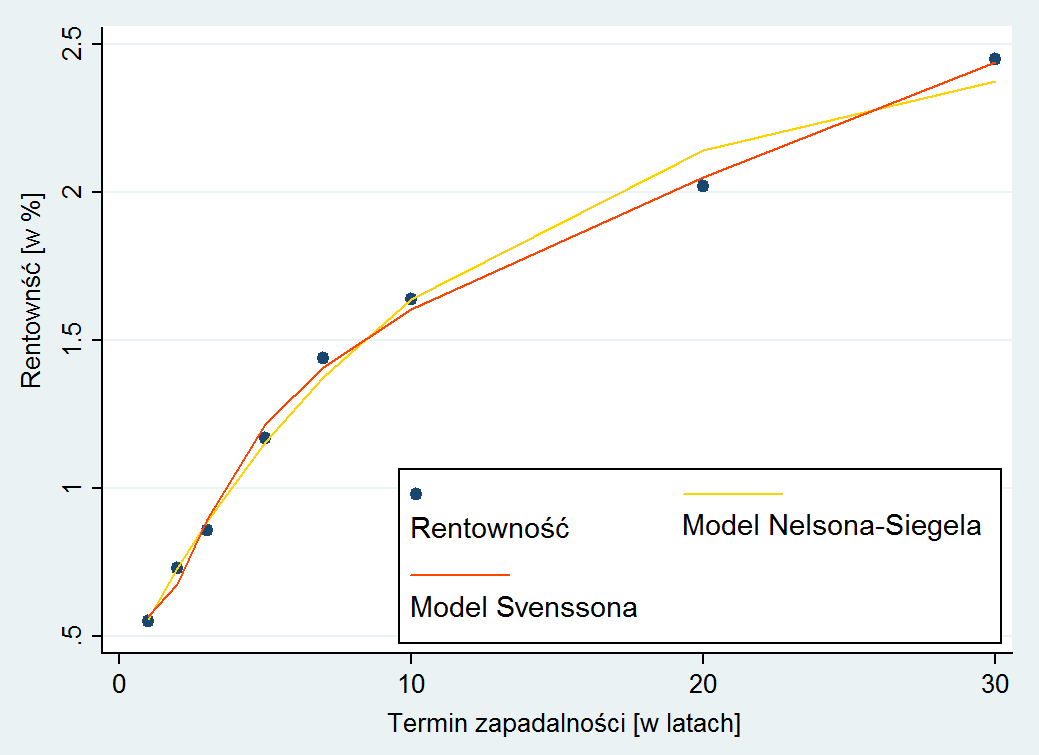
\includegraphics[height=4in]{Porownanie}
  \captionsetup{format=hang}
   \caption{Porównanie krzywych dochodowości amerykańskich obligacji skarbowych uzyskanych z~modelu Nelsona-Siegela i~modelu~Svenssona dla miesiąca czerwiec 2016}
\end{centering}
\begin{flushleft}
\hspace{1cm}\textit{\footnotesize{Źródło: Opracowanie własne.}} \\
\end{flushleft}
\end{figure}

Zaprezentowane powyżej modele posłużą w~bieżącej części rozdziału do wyznaczenia miesięcznych krzywych dochodowości. Ich komponenty zostały oszacowane przy pomocy Nieliniowej Metody Najmniejszych Kwadratów (ang. \textit{Non-linear Least Squares Method - NLSM}), przy parametrach początkowych: $\beta_0$ = 0, $\beta_1$ = 0, $\beta_2$ = 0, $\beta_3$ = 0, $\tau_1 = 1$, $\tau_2 = 1$. W~przypadku większości krzywych dochodowości wyznaczonych przez zaprezentowane powyżej modele lepiej dopasowane wizualnie okazały się krzywe uzyskane z~modelu Svenssona. Dobrym przykładem różnicy w~dopasowaniach modeli jest miesięczna krzywa dochodowości z~czerwca 2016~roku (\hyperlink{fig1}{wykres 1}). Jak wynika z~analizy powyższego wykresu krzywa uzyskana z~modelu Svenssona niemal idealnie przecina każdy z~punktów rentowności, krzywa wyliczona z~modelu Nelsona-Siegela nie jest tak dokładna. 

\vspace{0.25cm}
\hypertarget{fig2}{}
\begin{figure}[h]
\begin{centering}
  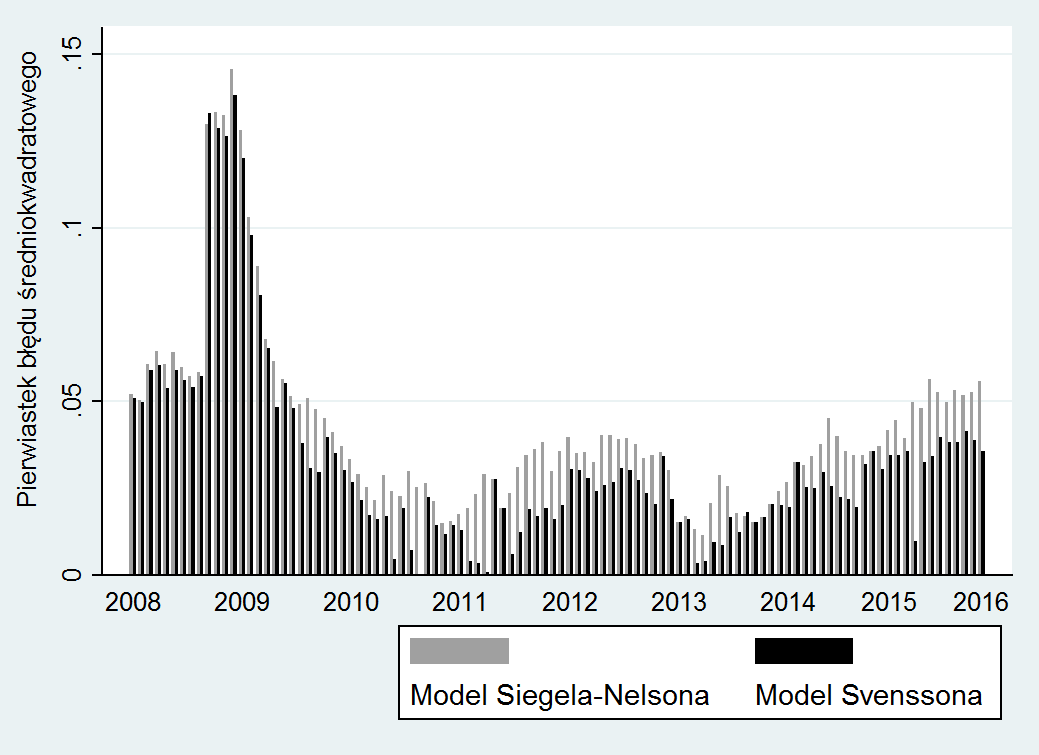
\includegraphics[height=4in]{RMSE}
  	\captionsetup{format=hang}
    \caption{Błędy RMSE uzyskane z~modelu Nelsona-Siegela i~modelu Svenssona dla krzywych dochodowości amerykańskich obligacji skarbowych w~latach 2008-2016}      
\end{centering}
\begin{flushleft}
\hspace{1cm}\textit{\footnotesize{Źródło: Opracowanie własne.}} \\
\end{flushleft}
\vspace{-0.5cm}
\end{figure}

Aby ostatecznie stwierdzić, który model jest lepiej dopasowany do sposobu kształtowania się rentowności obligacji skarbowych Stanów Zjednoczonych wyliczono pierwiastki błędów średniokwadratowych (ang. \textit{Root Mean Square Error - RMSE}) obu modeli zdefiniowane jako odchylenie krzywych wyestymowanych za pomocą analizowanych modeli od faktycznych rentowności (patrz \hyperlink{fig2}{wykres 2}). Kryterium minimalizacji pierwiastka błędu średniokwadratowego jednoznacznie wskazuje na konieczność wyboru modelu Svenssona, gdyż niemal w~całym badanym okresie (poza nielicznymi miesiącami) generuje on krzywe dochodowości z~niższym \acs{RMSE} niż model Nelsona-Siegela. Analizę wykresu pierwiastków błędów średniokwadratowych potwierdzają ich statystyki opisowe zaprezentowane w~\hyperlink{tab1}{tabeli 2}. Całkowita suma błędów \acs{RMSE}, ich średnia i~mediana jednoznacznie wskazują, że lepiej dopasowanym modelem do danych jest model Svenssona, jedynie nieznacznie niższe odchylenie standardowe mogłoby sugerować model Nelsona-Siegla. Aby sprawdzić czy średnie błędy \acs{RMSE} z~obu modeli istotnie się pomiędzy sobą różnią przeprowadzono test Manna-Whitneya-Wilcoxona (\acs{MWW}) na równość średnich w~próbkach niezależnych, który wykazał konieczność odrzucenia hipotezy zerowej o~równości średnich błędów \acs{RMSE} obu porównywanych modeli. Oznacza to, iż średnie błędy z~modelu Nelsona-Siegiela są istotnie wyższe niż średnie błędy z~modelu Svenssona. Biorąc pod uwagę zarówno analizę graficzną, statystyki opisowe, jak i~wynik testu statystycznego zdecydowano, iż do dalszych analiz przeprowadzanych w~tej pracy posłuży model Svenssona, jako model lepiej dopasowany do specyfiki amerykańskich papierów dłużnych. 

\hypertarget{tab1}{}
\begin{table}[!ht]
\rowcolors{2}{lightgray}{white}
\captionsetup{format=hang, position=top}
\caption{Statystyki opisowe błędów RMSE z~modelu Nelsona-Siegiela i modelu Svenssona oraz statystyka testowa MWW na równość średnich RMSE obu modeli}
\begin{tabular}{M{4.5cm}M{2.5cm}M{2.5cm}}
\toprule
\textbf{Cecha RMSE} & \textbf{Model_NS} & \textbf{Model_Svens}\\
\midrule
Suma & 4,3273 & 3,3884\\
Średnia & 0,0424 & 0,0332\\
Mediana & 0,0358 & 0,0268\\
Odchylenie Standardowe & 0,0262 & 0,0277\\
Statystyka testowa \acs{MWW} & \multicolumn{2}{c}{-3,966$^{***}$} \\
\bottomrule
\rowcolor{white!50}
\multicolumn{3}{m{10.5cm}}{\scriptsize Liczba gwiazdek wskazuje na jakim poziomie istotności należy odrzucić hipotezę zerową - w~przypadku testu Manna-Whitneya-Wilcoxona o~równości średnich w~próbkach niezależnych: 10\% ($^{*}$), 5\% ($^{**}$), 1\% ($^{***}$).}
\end{tabular}
\begin{flushleft}
\hspace{1cm}\textit{\footnotesize{Źródło: Opracowanie własne.}} \\
\end{flushleft}
\vspace{-0.5cm}
\end{table} 

\hyperlink{fig3}{Wykres 3} przedstawia kształtowanie się najważniejszych komponentów krzywej dochodowości obligacji skarbowych Stanów Zjednoczonych dla lat 2008-2016. Pierwszym istotnym komponentem krzywej dochodowości jest składnik krótkoterminowy ($\beta_0$ + $\beta_1$), oscylował on w~latach 2008-2011~wokół wartości -1\%, by w~kolejnych pięciu latach systematycznie rosnąć osiągając w~rezultacie wartość zbliżoną do 2\%. W~związku z~tym, iż sumę $\beta_0 + \beta_1$ interpretuje się jako bieżącą stopę oprocentowania lokaty overnight ($lim_{m->0}$ $R(m) = \beta_0$ + $\beta_1$) zachowanie tego wskaźnika może wskazywać, iż w~pierwszych trzech latach kryzysu Rezerwie Federalnej udało się utrzymać krótki koniec krzywej dochodowości na poziomie ujemnym, by w~kolejnych latach utracić wpływ na zachowanie się tego fragmentu krzywej dochodowości amerykańskich papierów dłużnych. 

\hypertarget{fig3}{}
\begin{figure}[h]
\vspace{0.25cm}
\begin{centering}
  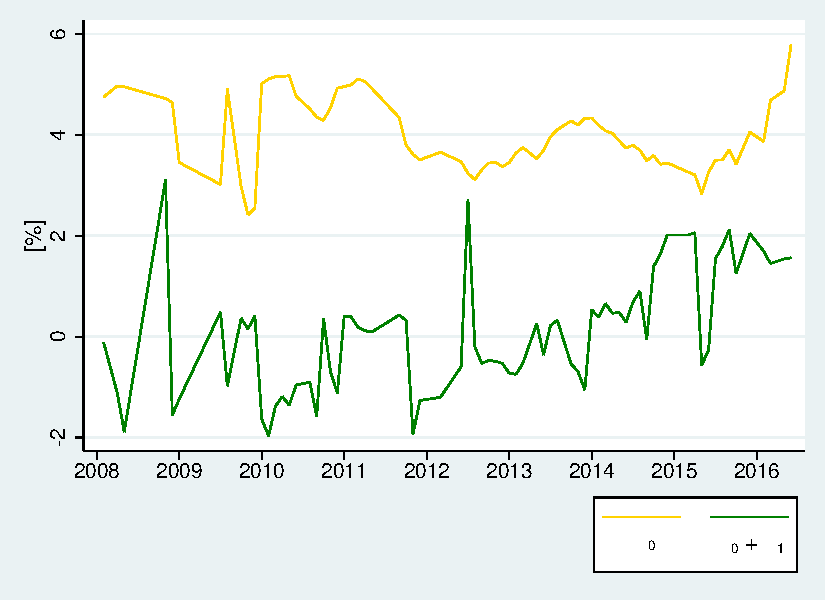
\includegraphics[height=4in]{Rysunki//Bety}
    \captionsetup{format=hang}
    \caption{Najważniejsze oszacowania krzywej dochodowości amerykańskich obligacji skarbowych wyliczone za pomocą modelu Svenssona dla lat 2008-2016}
\end{centering}
\begin{flushleft}
\hspace{1cm}\textit{\footnotesize{Źródło: Opracowanie własne.}} \\
\end{flushleft}
\vspace{-0.25cm}
\end{figure} 

Drugim istotnym komponentem krzywej dochodowości jest składnik długoterminowy $\beta_0$, który zgodnie z~\hyperlink{fig3}{wykresem 3}~początkowo oscylował wokół wartości równej 4\%, by od 2011~roku stopniowo ulegać osłabieniu osiągając w~połowie 2015~roku poziom zbliżony do 3\%. Z~kolei ostatnie dwa lata badania to dynamiczny wzrost parametru $\beta_0$ uwieńczony osiągnięciem poziomu zbliżonego do 6\%. Komponent $\beta_0$ interpretowany jest jako stopa, do której w~długim okresie dążą wszystkie stopy z~całej długości krzywej dochodowości ($lim_{m-> \infty}$ $R(m) = \beta_0$). Zachowanie tego parametru w~latach 2008-2016~może wskazywać, iż Rezerwie Federalnej udało się realnie obniżyć stopy długoterminowe dopiero po 2012~roku, czyli po ponad 3~latach stosowania luzowania ilościowego i~wydaniu blisko 2~bilionów dolarów. Obniżka ta została jednak odwrócona w~momencie, w~którym zaczęły się pojawiać pierwsze sygnały od członków \acs{FED} o~możliwym wyhamowaniu programu luzowania ilościowego. Kolejnym etapem badania będzie sprawdzenie, czy decyzje Rezerwy Federalnej miały faktyczny, statystycznie istotny, wpływ na kształt krzywej dochodowości obligacji skarbowych w~latach 2008-2016~wyznaczony za pomocą modelu Larsa E.O. Svenssona jako modelu najlepiej dopasowanego do danych.

\phantomsection	% do hiperlinków dla sekcji w spisie treści
\subsection*{\normalsize{3.1.2. Reakcja krzywej dochodowości na zmiany polityki monetarnej FED}}
\addcontentsline{toc}{subsection}{3.1.2. Reakcja krzywej dochodowości na zmiany polityki monetarnej FED}

W~badaniu reakcji krzywej dochodowości obligacji skarbowych Stanów Zjednoczonych na zmiany polityki monetarnej Rezerwy Federalnej postanowiono posłużyć się analizą graficzną średniomiesięcznych krzywych dochodowości wspartą testami na istotność różnic pomiędzy średnimi dziennymi rentownościami obligacji przed i~po ogłoszeniu komunikatu władz monetarnych (\textit{event study}). W~tym celu zidentyfikowano 10~najważniejszych komunikatów dotyczących niekonwencjonalnej polityki pieniężnej wygłoszonych przez członków amerykańskich władz monetarnych w~latach 2008-2016, które mogły istotnie wpłynąć na kształt krzywej dochodowości w~tym okresie. Daty tych wypowiedzi oraz ich skrócona treść zostały przedstawione w~\hyperlink{tab2}{tabeli 3}. 

Kolejnym etapem badania było sprawdzenie czy zaprezentowane w~\hyperlink{tab2}{tabeli 3} komunikaty istotnie wpłynęły, w~krótkim terminie, na kształt krzywej dochodowości reprezentowany przez średnie dzienne rentowności amerykańskich obligacji skarbowych. Założono w~tym momencie, iż już samo ogłoszenie zmian w~polityce monetarnej ma realny wpływ na oczekiwania uczestników rynku i~przejawia się za pomocą zmian rentowności obligacji skarbowych w~kolejnych dniach notowań następujących po ogłoszeniu komunikatu (kanał transmisji impulsów polityki monetarnej dotyczący oczekiwań uczestników rynku). Natomiast wdrożenie polityki (fizyczny skup aktywów) powinien być najlepiej odzwierciedlony w~zmianie kształtu krzywych dochodowości w~kolejnych miesiącach stosowania polityki (kanał pozostałych cen aktywów). 

Aby móc określić statystyczną istotność wpływu każdego z~przedstawionych w~\hyperlink{tab2}{tabeli 3}~komunikatów na średnie dzienne rentowności amerykańskich obligacji skarbowych przeprowadzono testy na równość średniej w~próbkach zależnych. Dla każdego z~komunikatów wydzielono dwa okna obserwacyjne - pierwsze z~obserwacjami poprzedzającymi, do miesiąca wstecz, komunikat (Okno 1) i~drugie z~obserwacjami następującymi1 do miesiąca po komunikacie, w~tym z~dnia komunikatu (Okno 2). Zastosowano tak wąskie okna obserwacji aby zapewnić, iż na poziomy rentowności obligacji w~tych oknach badawczych istotnie wpływać będą jedynie badane komunikaty (minimalny okres pomiędzy posiedzeniami \acs{FOMC} wynosi jeden miesiąc) a~nie inne wydarzenia rynkowe. W~rezultacie otrzymano po dwie próbki dla każdego komunikatu (przed i~po) zawierające po 21~obserwacji każda (średnia liczba dni notowań w~miesiącu). Obserwacje uzyskane w~próbkach reprezentują średni poziom rentowności dłużnych papierów skarbowych USA w~danym dniu notowań zdefiniowany jako średnia arytmetyczna z~rentowności obligacji o~ośmiu długościach od 1~roku do~30 lat (1-,~2-,~3-,~5-,~7-, 10-,~20-~i~30-letnie).

\hypertarget{tab2}{}
\begin{table}[H]
\rowcolors{2}{lightgray}{white}
\captionsetup{format=hang, position=top}
\caption{Daty i~skrócona treść najważniejszych komunikatów Rezerwy Federalnej dotyczących niekonwencjonalnej polityki monetarnej  w~latach 2008-2016}
\begin{tabular}{M{2.75cm}M{12.5cm}}
\toprule
\textbf{Data komunikatu} & \textbf{Skrócona treść komunikatu Rezerwy Federalnej}\\
\midrule
\hypertarget{kom1}{Komunikat 1:} 25.11.2008 & Ogłoszenie pierwszego programu luzowania ilościowego (\acs{QE}1) - plan zakupu: obligacji przedsiębiorstw sponsorowanych przez rząd (\acs{GSE}) o~wartości 100~miliardów dolarów oraz hipotecznych listów zastawnych (\acs{ABS}) o~wartości 500~miliardów.\cite{Fed09}   \\
\hypertarget{kom2}{Komunikat 2:} 18.03.2009 & Rozszerzenie program \acs{QE}1 - plan zakupu do końca marca 2010~roku 1,25~biliona hipotecznych listów zastawnych oraz 300~miliardów długoterminowych amerykańskich obligacji skarbowych.\cite{Fed10} \\
\hypertarget{kom3}{Komunikat 3:} 27.08.2010 & Szef Rezerwy Federalnej Ben Bernanke w~corocznej przemowie w~Jackson Hole wskazuje na możliwość przeprowadzenia kolejnego programu luzowanie ilościowego.\cite{bernanke11}\\
\hypertarget{kom4}{Komunikat 4:} 03.11.2010 & Ogłoszenie drugiego programu luzowania ilościowego (\acs{QE}2) - plan zakupu 600~miliardów amerykańskich długoterminowych obligacji skarbowych do końca czerwca 2011~roku.\cite{Fed12} \\
\hypertarget{kom5}{Komunikat 5:} 21.09.2011 & Ogłoszenie programu Operacja Twist - planu wydłużenie średniej duracji portfela \acs{FED} poprzez zakup do końca czerwca 2012~roku amerykańskich obligacji skarbowych o~wartości 400~miliardów dolarów z~zapadalnością od 6.~do~30. lat przy jednoczesnej sprzedaży obligacji krótszych niż trzyletnie o~takiej samej wartości.\cite{Fed13} \\
\hypertarget{kom6}{Komunikat 6:} 13.09.2012 & Ogłoszenie trzeciego programu luzowania ilościowego (\acs{QE}3) - plan regularnych, miesięcznych zakupów hipotecznych listów zastawnych o~wartości 40~miliardów dolarów bez określenia konkretnej daty zakończenia programu. Kontynuowanie operacji wydłużania duracji portfela obligacji skarbowych (\acs{OT}).\cite{Fed14}\\
\hypertarget{kom7}{Komunikat 7:} 12.12.2012 & Rozszerzenie programu \acs{QE}3 - poza kontynuowaniem regularnych zakupów hipotecznych listów zastawnych w~tempie 40~miliardów miesięcznie postanowiono dokonywać również zakupu długoterminowych amerykańskich obligacji skarbowych o~wartości 45~miliardów miesięcznie.\cite{Fed15}\\
\hypertarget{kom8}{Komunikat 8:} 19.06.2013 & Zapowiedź ograniczenia programu \acs{QE}3 (ang. \textit{Taper Tantrum - TT}) - wypowiedź przewodniczącego Rezerwy Federalnej sugerująca możliwość ograniczenia tempa skupu aktywów ze względu na poprawiająca się sytuację ekonomiczną amerykańskiej gospodarki (rozpoczęcie procesu wycofywania się z~niekonwencjonalnej polityki pieniężnej).\cite{bernanke18}\\
\hypertarget{kom9}{Komunikat 9:} 18.12.2013 & Rozpoczęcie ograniczania programu \acs{QE}3 - plan zmniejszania miesięcznej wartości kupowanych aktywów o~10 miliardów dolarów na każdym posiedzeniu w~2014 roku.\cite{Fed16}\\
\hypertarget{kom10}{Komunikat 10:} 29.10.2014 & Ostateczne zakończenie trzeciego programu luzowania ilościowego po zgromadzeniu papierów wartościowych o~wartości blisko 4,5~biliona dolarów w~bilansie Rezerwy Federalnej.\cite{Fed17}\\
\bottomrule
\end{tabular}
\begin{flushleft}
\hspace{1cm}\textit{\footnotesize{Źródło: Opracowanie własne.}} \\
\end{flushleft}
\vspace{-0.5cm}
\end{table} 

Większość uzyskanych próbek pochodziło z~rozkładu normalnego, badanego przy pomocy testu Shapiro-Wilka (\acs{SW}) odpowiedniego dla małych prób nieprzekraczających 50~obserwacji. Wyjątek stanowił okres 21 dni po ogłoszeniu \hyperlink{kom10}{komunikatu nr 10}, który okazał się nie posiadać rozkładu zbliżonego do normalnego. Dla tak zdefiniowanych próbek przeprowadzono testy: parametryczny test T~oraz nieparametryczny test Wilcoxona.

\vspace{0.25cm}
\hypertarget{tab3}{}
\begin{table}[!ht]
\rowcolors{4}{lightgray}{white}
\captionsetup{format=hang, position=top}
\caption{Statystyki testowe testów na normalność (SW) oraz na równość średnich w~próbach zależnych (T-Test i~Wilcoxon), a~także zmiana średniej rentowności dla 10~najważniejszych komunikatów Rezerwy Federalnej z~lat 2008-2016}
\begin{tabular}{
M{2.5cm}
S[table-format=3.3,table-space-text-post=$^{***}$]
S[table-format=3.3,table-space-text-post=$^{***}$]
S[table-format=3.3,table-space-text-post=$^{***}$]
S[table-format=3.3,table-space-text-post=$^{***}$]
M{2.5cm}
}
\toprule
\textbf{Numer} & \textbf{Statystyka} & \textbf{Statystyka} & \textbf{Statystyka} & \textbf{Statystyka} & \textbf{Zmiana}\\
\textbf{komunikatu} & {\textbf{testowa}} & {\textbf{testowa}} & {\textbf{testowa}} & {\textbf{testowa}} & \textbf{średniej}\\
\textbf{FED} & {\textbf{SW (Okno 1)}} & {\textbf{SW (Okno 2)}} & {\textbf{T-Test}} & {\textbf{Wilcoxon}}& \textbf{rentowności}\\
\midrule
Komunikat 1  & 0,914$^{*}$ &  0,953 &  24,932$^{***}$ &    4,015$^{***}$  &    {-86 p.b.}\\
Komunikat 2  &  0,947 &  0,970 &   5,236$^{***}$ &    3,493$^{***}$  &    {-10 p.b.}\\
Komunikat 3  & 0,946 & 0,983 &   2,307$^{**}$  &    1,547          &      {-}\\
Komunikat 4  &  0,963 & 0,921$^{*}$ & -10,122$^{***}$ &   -3,998$^{***}$  &    {+21 p.b.}\\
Komunikat 5  &  0,954 & 0,937 &   1,495         &    1,373          &        {-} \\
Komunikat 6  & 0,943 & 0,951 &  -1,282         &   -1,269          &        {-} \\
Komunikat 7  & 0,962 & 0,948 & -10,307$^{***}$ &   -4,015$^{***}$  &    {+12 p.b.}\\
Komunikat 8  &  0,914$^{*}$ & 0,953 & -17,909$^{***}$ &   -4,015$^{***}$  &    {+24 p.b.}\\
Komunikat 9  & 0,943 &  0,915$^{*}$ &  -7,474$^{***}$ &   -4,015$^{***}$  &    {+11 p.b.}\\
Komunikat 10 & 0,953 & 0,866$^{***}$ &  {-}    &   -1,251          &          {-} \\
\bottomrule
\multicolumn{6}{m{15cm}}{\scriptsize Liczba gwiazdek wskazuje na jakim poziomie istotności należy odrzucić hipotezę zerową - w~przypadku testu Shapiro-Wilka o~normalności rozkładu, w~przypadku T-Testu i~Wilcoxona o~równości średnich w~próbkach zależnych: 10\% ($^{*}$), 5\% ($^{**}$), 1\% ($^{***}$).}
\end{tabular}
\begin{flushleft}
\textit{\footnotesize{Źródło: Opracowanie własne.}} \\
\end{flushleft}
\vspace{-0.35cm}
\end{table} 

Wyniki testów na równość średnich w~próbkach zależnych zostały zaprezentowane w~\hyperlink{tab3}{tabeli 4}. Jej analiza wskazuje na statystyczną istotność na 99\%-owym poziomie ufności sześciu komunikatów: \hyperlink{kom1}{1}, \hyperlink{kom2}{2}, \hyperlink{kom4}{4}, \hyperlink{kom7}{7}, \hyperlink{kom8}{8} oraz \hyperlink{kom9}{9}. \hyperlink{kom3}{Trzeci komunikat} okazał się istotny na 95\%-owym poziomie istotności tylko w~teście T, dlatego też nie został w~niniejszej pracy uznany za istotnie wpływający na kształt krzywej dochodowości. Dla komunikatów \hyperlink{kom5}{5.} i~\hyperlink{kom6}{6.} oba testy wskazały na brak konieczności odrzucenia hipotezy zerowej o~równości średnich w~próbkach zależnych na akceptowalnym poziomie istotności (5\%) - co oznacza, iż nie wpłynęły one istotnie na średnią rentowność amerykańskich obligacji skarbowych. Dla \hyperlink{kom10}{komunikatu 10.} ze względu na brak normalności jednej z~próbek można było przeprowadzić tylko test Wilcoxona, wskazał on na brak konieczności odrzucenia hipotezy zerowej o~równości średniej w~próbkach zależnych na akceptowalnym poziomie istotności - komunikat okazał się statystycznie nieistotny. 

\hyperlink{tab3}{Tabela 4}~poza statystykami testowymi prezentuje również skalę zmiany średniej rentowności dla komunikatów statystycznie istotnych. Jak wynika z~tabeli tylko dwa pierwsze komunikaty wpłynęły istotnie na natychmiastowy spadek średniej rentowności amerykańskich obligacji skarbowych. Tymi komunikatami było rozpoczęcie pierwszego luzowania ilościowego (-86~p.b.) oraz jego rozszerzenie (-10~p.b.) - co jest zgodne z~obserwacjami przedstawionymi w~artykule J. Gagnon, M. Raskin, J.Remache oraz B. Sack \cite{gagnon34}, omówionym w drugim rozdziale niniejszej pracy. Pozostałe komunikaty przedstawione w~\hyperlink{tab3}{tabeli 3} albo okazały się statystycznie nieistotne albo wpłynęły na nieznaczny wzrost średnich rentowności przynajmniej w~krótkoterminowej perspektywie. Jest to całkowicie zrozumiałe w~przypadku informacji o~ograniczeniu skali zakupów obligacji skarbowych (komunikaty \hyperlink{kom8}{8} i~\hyperlink{kom9}{9}) jednak zapowiedzi rozszerzenia skali niekonwencjonalnych programów (komunikaty \hyperlink{kom4}{4} i~\hyperlink{kom7}{7}) powinny prowadzić do spadku rentowności amerykańskich obligacji skarbowych. 

\vspace{0.25cm}
\hypertarget{fig4}{}
\begin{figure}[h]
\begin{centering}
  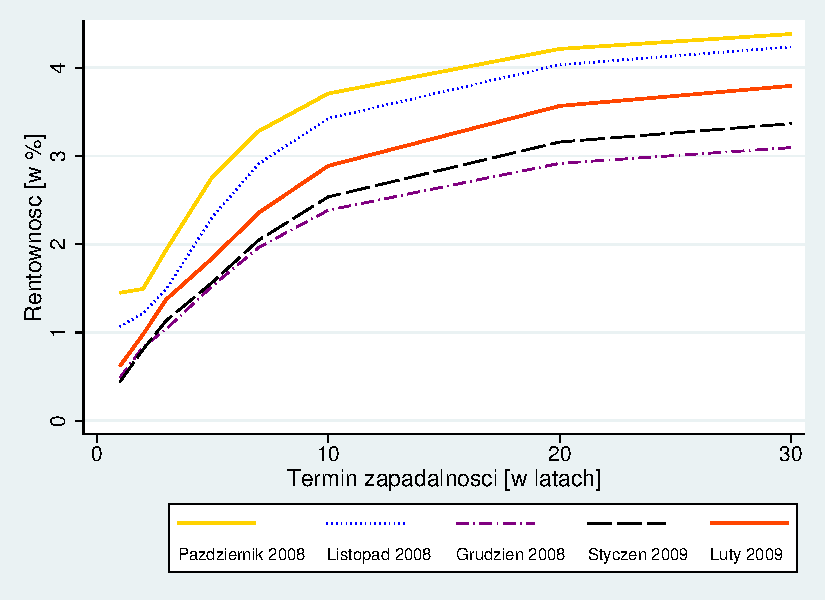
\includegraphics[height=4in]{krzywa1}
    \captionsetup{format=hang}
    \caption{Reakcja krzywej dochodowości na ogłoszenie \protect\hyperlink{kom1}{komunikatu 1} (rozpoczęcie QE1)}
\end{centering}
\begin{flushleft}
\hspace{1cm}\textit{\footnotesize{Źródło: Opracowanie własne.}} \\
\end{flushleft}
\vspace{-0.5cm}
\end{figure}

Po zbadaniu krótkoterminowej reakcji krzywej dochodowości na ogłaszanie kolejnych programów niekonwencjonalnej polityki pieniężnej w~dalszej analizie skupiono się na kształcie krzywych dochodowości w~nieco dłuższym, trzymiesięcznym okresie, odnosząc swe analizy do miesiąca poprzedzającego miesiąc ogłoszenia komunikatu. \hyperlink{fig4}{Wykres 4}~prezentuje kształt krzywej dochodowości dla miesiąca poprzedzającego decyzję Rezerwy Federalnej o~rozpoczęciu pierwszego programu luzowania ilościowego oraz krzywe z~kolejnych czterech miesięcy następujących po ogłoszeniu \hyperlink{kom1}{komunikatu 1}. Z~wykresu wynika, iż ogłoszenie zastosowania niekonwencjonalnej polityki pieniężnej mogło spowodować wyraźne spłaszczenie się krzywej dochodowości w~perspektywie 4~miesięcy na całej jej długości od o~około 50~punktów bazowych na krótkim jej końcu aż do 1~punktu procentowego w~jej dalszym fragmencie\footnote{Warto w~tym miejscu wspomnieć, że 16.~grudniu 2008 roku amerykańskie władze monetarne postanowiły zakończyć trwającą od sierpnia 2007 roku serię obniżek stopy funduszy federalnych ustanawiając dla niej przedział 0\%-0,25\%, co mogło mieć najsilniejszy wpływ na krótki koniec krzywej dochodowości.}. Wnioski te pokrywają się z~analizą przedstawioną we wcześniejszym fragmencie rozdziału gdzie krótkoterminowy wpływ \hyperlink{kom1}{komunikatu 1} na średnią rentowność wynosił około -84~punkty bazowe - w~perspektywie 4~miesięcy wpływ ten spadł do -73~punktów bazowych.

\vspace{0.25cm}
\hypertarget{fig5}{}
\begin{figure}[h]
\begin{centering}
  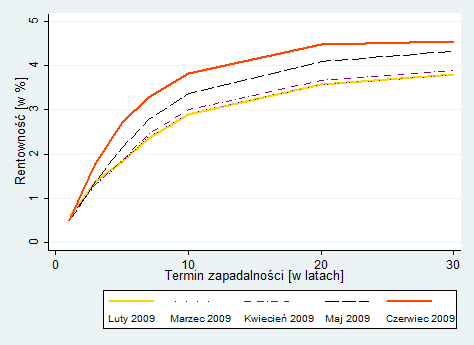
\includegraphics[height=4in]{krzywa2}
    \captionsetup{format=hang}
    \caption{Reakcja krzywej dochodowości na ogłoszenie \protect\hyperlink{kom2}{komunikatu 2} (rozszerzenie QE1)}
\end{centering}
\begin{flushleft}
\hspace{1cm}\textit{\footnotesize{Źródło: Opracowanie własne.}} \\
\end{flushleft}
\vspace{-0.5cm}
\end{figure}

Ogłoszenie komunikatu o~rozszerzeniu pierwszego programu luzowania ilościowego 18. marca 2009~roku przynosi zupełnie inne obserwacje (\hyperlink{fig5}{wykres 5}). Analiza \hyperlink{fig5}{wykresu 5} wskazuje, iż ogłoszenie \hyperlink{kom2}{komunikatu 2} mogło co najwyżej chwilowo wyhamować obserwowane od stycznia 2009~wzrosty rentowności amerykańskich obligacji skarbowych (-10 b.p reakcji dziennych krzywych), które już w~czerwcu 2009~wróciły do poziomów z~października 2008. Taka reakcja krzywej dochodowości wydaje się sprzeczna z~oczekiwaniami - ogłoszenie bezprecedensowego planu zakupu przez Rezerwę Federalną długoterminowych amerykańskich obligacji skarbowych o~wartości 300~miliardów dolarów powinno wyraźnie wzmocnić popyt rynkowy i~bezpośrednio wpłynąć na wzrost cen obligacji~a tym samym na obniżenie ich rentowności. Nie miało to jednak miejsca - rentowności w~kolejnych miesiącach wzrastały nie zważając na znaczące zakupy amerykańskich obligacji skarbowych przez Rezerwę Federalną.

\vspace{0.25cm}
\hypertarget{fig6}{}
\begin{figure}[h]
\begin{centering}
  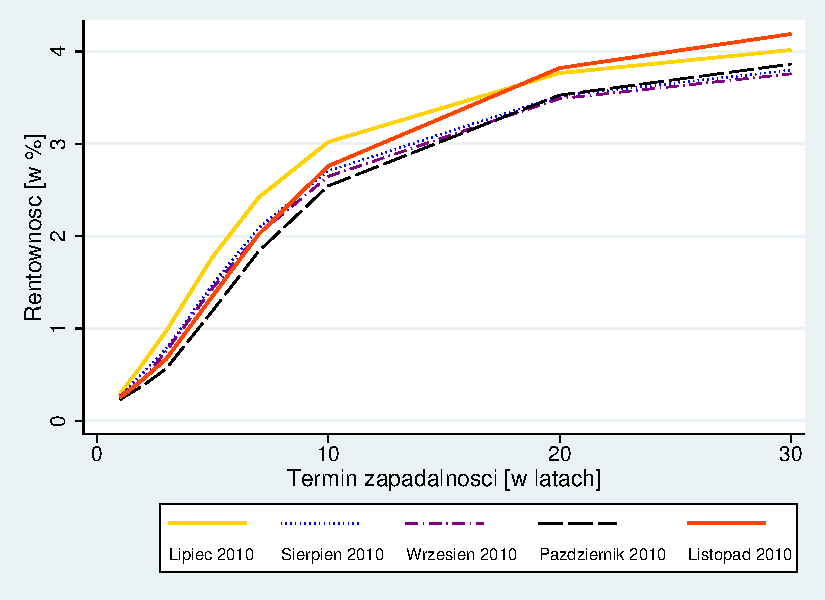
\includegraphics[height=4in]{krzywa3}
    \captionsetup{format=hang}
    \caption{Reakcja krzywej dochodowości na ogłoszenie \protect\hyperlink{kom3}{komunikatu 3} (zapowiedź QE2)}
\end{centering}
\begin{flushleft}
\hspace{1cm}\textit{\footnotesize{Źródło: Opracowanie własne.}} \\
\end{flushleft}
\vspace{-0.5cm}
\end{figure}

\hyperlink{fig6}{Wykres 6}~potwierdza wnioski płynące z~analizy dziennych rentowności - od lipca 2010~roku do listopada 2010~roku krzywa dochodowości praktycznie nie zmieniła swojego kształtu poza delikatnym spłaszczeniem się (około -10 punktów bazowych) we fragmencie pomiędzy rokiem a~dziesięcioma latami. Mogłoby to wskazywać, iż \hyperlink{kom3}{komunikat 3} był neutralny dla uczestników rynku dłużnych papierów skarbowych w~Stanach Zjednoczonych. Co oznacza, iż albo został on ujęty wcześniej w~cenach, albo obserwacje pierwszego programu luzowania ilościowego kazały sądzić inwestorom, iż drugi taki program nie będzie miał znaczącego wpływu na rynek.

\vspace{0.5cm}
\hypertarget{fig7}{}
\begin{figure}[H]
\centering
\captionsetup{format=hang}
\caption{Reakcje krzywych dochodowości na ogłoszenie komunikatów \protect\hyperlink{kom4}{4} oraz \protect\hyperlink{kom5}{5}}
\begin{subfigure}{.5\textwidth}
\hspace{-3cm}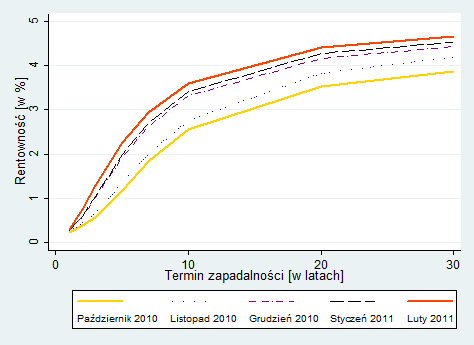
\includegraphics[height=4in]{krzywa4}
 \caption{\protect\hyperlink{kom4}{Komunikat 4} (rozpoczęcie QE2)}
\hypertarget{fig7}{}
\vspace*{\floatsep} % przerwa między wykresami
\end{subfigure}
\begin{subfigure}{.5\textwidth}
\hspace{-3cm}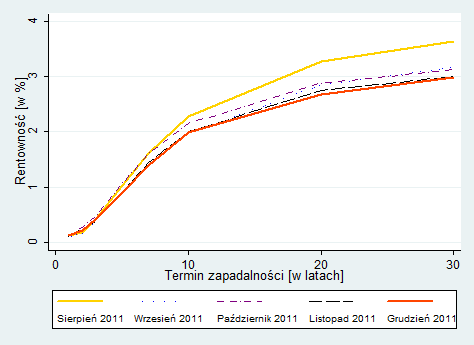
\includegraphics[height=4in]{krzywa5}
\caption{\protect\hyperlink{kom5}{Komunikat 5} (rozpoczęcie OT)}
\end{subfigure}
\begin{flushleft}
\hspace{1cm}\textit{\footnotesize{Źródło: Opracowanie własne.}} \\
\end{flushleft}
\vspace{-0.5cm}
\end{figure}

Na \hyperlink{fig7}{wykresie 7}~zaprezentowane są krzywe dochodowości w~kolejnych miesiącach po ogłoszeniu komunikatów \hyperlink{kom4}{4} i~\hyperlink{kom5}{5}. W~obu przypadkach potwierdzają się wnioski płynące z~analizy zmian dziennych rentowności. Tuż po rozpoczęciu \acs{QE}2 krzywa dochodowości wzrosła o~około 25~p.b. by do lutego 2011~roku wzrosnąć o~kolejne 50~p.b. Rozpoczęcie operacji Twist nie wpłynęło istotnie na rentowności obligacji skarbowych, widać jedynie ich delikatny spadek (-20 p.b.) na długim końcu krzywej w~stosunku do miesiąca przed ogłoszeniem tego programu.

\vspace{0.25cm}
\hypertarget{fig8}{}
\begin{figure}[h]
\begin{centering}
  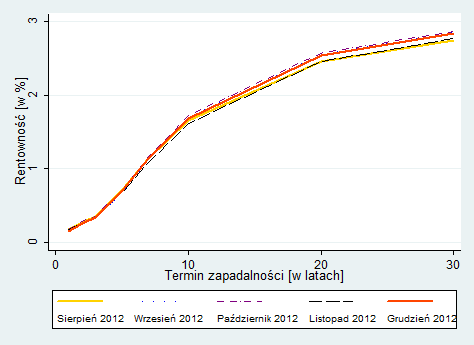
\includegraphics[height=4in]{krzywa6}
    \captionsetup{format=hang}
    \caption{Reakcja krzywej dochodowości na ogłoszenie \protect\hyperlink{kom6}{komunikatu 6} (rozpoczęcie QE3)}
\end{centering}
\begin{flushleft}
\hspace{1cm}\textit{\footnotesize{Źródło: Opracowanie własne.}} \\
\end{flushleft}
\vspace{-0.5cm}
\end{figure}

Wnioski płynące z~analizy \hyperlink{fig8}{wykresu 8} są tożsame z~wnioskami płynącymi z~analizy wpływu \hyperlink{kom6}{komunikatu 6} na dzienne rentowności obligacji skarbowych - kształt krzywej dochodowości pozostawał praktycznie bez zmian pomiędzy sierpniem 2012~a grudniem 2012~pomimo ogłoszenia kolejnego, trzeciego już, programu luzowania ilościowego. Brak reakcji krzywej dochodowości może tłumaczyć fakt, iż \acs{QE}3~początkowo zakładało skup hipotecznych listów zastawnych w~tempie 40~miliardów dolarów miesięcznie, a~nie bezpośrednio obligacji skarbowych. Kontynuowana była jednak program wydłużania duracji portfela Rezerwy Federalnej, który w~intencji amerykańskich władz monetarnych miał wywoływać spadek rentowności długoterminowych obligacji skarbowych.

\vspace{0.5cm}
\hypertarget{fig9}{}
\begin{figure}[H]
\centering
\captionsetup{format=hang}
\caption{Reakcje krzywych dochodowości na ogłoszenie komunikatów \protect\hyperlink{kom7}{7} oraz \protect\hyperlink{kom8}{8}}
\begin{subfigure}{.5\textwidth}
\hspace{-3cm}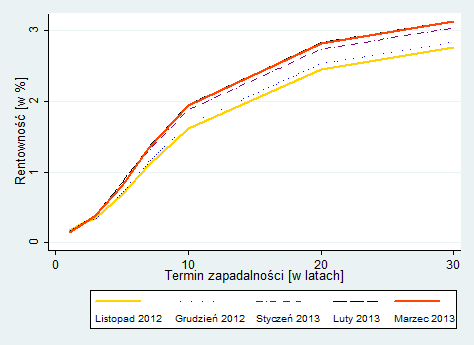
\includegraphics[height=4in]{krzywa7}
 \caption{\protect\hyperlink{kom7}{Komunikat 7} (rozszerzenie QE3)}
\hypertarget{fig10}{}
\vspace*{\floatsep} % przerwa między wykresami
\end{subfigure}
\begin{subfigure}{.5\textwidth}
\hspace{-3cm}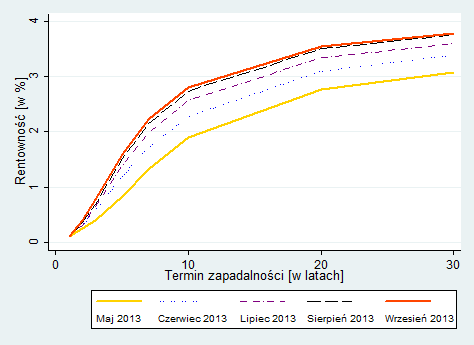
\includegraphics[height=4in]{krzywa8}
\caption{\protect\hyperlink{kom8}{Komunikat 8} (zapowiedź ograniczenia QE3)}
\end{subfigure}
\begin{flushleft}
\hspace{1cm}\textit{\footnotesize{Źródło: Opracowanie własne.}} \\
\end{flushleft}
\vspace{-0.5cm}
\end{figure}

Krzywe dochodowości po ogłoszeniu komunikatów \hyperlink{kom7}{7} i~\hyperlink{kom8}{8} kształtowały się bardzo podobnie (patrz \hyperlink{fig9}{wykresu 9}), pomimo, iż pierwszy z~nich dotyczył rozszerzenia skali zakupów obligacji skarbowych, a~drugi zapowiadał ich ograniczenie. Obie krzywe odnotowały wzrosty pierwsza o~około 30~p.b. a~druga o~około 50~p.b. z~tym, że w~przypadku tej drugiej wzrosty były dużo wyraźniejsze dla rentowności od roku do dziesięciu lat. 

\vspace{0.25cm}
\hypertarget{fig11}{}
\begin{figure}[h]
\begin{centering}
  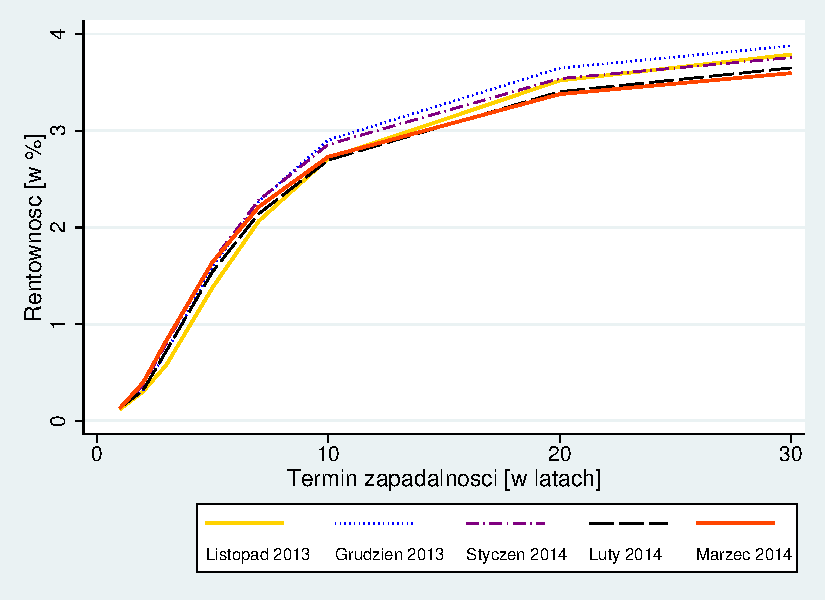
\includegraphics[height=4in]{krzywa9}
    \captionsetup{format=hang}
    \caption{Reakcja krzywej dochodowości na ogłoszenie \protect\hyperlink{kom9}{komunikatu 9} (ograniczenie QE3)}
\end{centering}
\begin{flushleft}
\hspace{1cm}\textit{\footnotesize{Źródło: Opracowanie własne.}} \\
\end{flushleft}
\vspace{-0.5cm}
\end{figure}

Wbrew wnioskom płynącym z~pierwszej części podrozdziału, wydaje się, iż ogłoszenie \hyperlink{kom9}{komunikatu 9} nie odcisnęło swojego piętna na kształcie krzywej dochodowości - rentowności z~okresu listopad 2013 - marzec 2014~nie uległy zbyt istotnym zmianom. Badanie reakcji krótkoterminowej wskazywało na nieznaczny wzrost o~około~11~p.b., który jest również zauważalny na \hyperlink{fig11}{wykresie 10}, jednak w~kolejnych miesiącach wzrost ten został całkowicie zniwelowany przez delikatne spłaszczenie się krzywej dochodowości. Można by domniemywać, iż ten komunikat był spodziewany przez rynek z~powodu kilku wcześniejszych wypowiedzi przewodniczącego Rezerwy Federalnej i~został ujęty już wcześniej w~wycenach amerykańskich obligacji skarbowych, dlatego też nie wywołał tak znaczącego efektu jak wcześniejsze zapowiedzi.\\

\vspace{0.25cm}
\hypertarget{fig12}{}
\begin{figure}[h]
\begin{centering}
  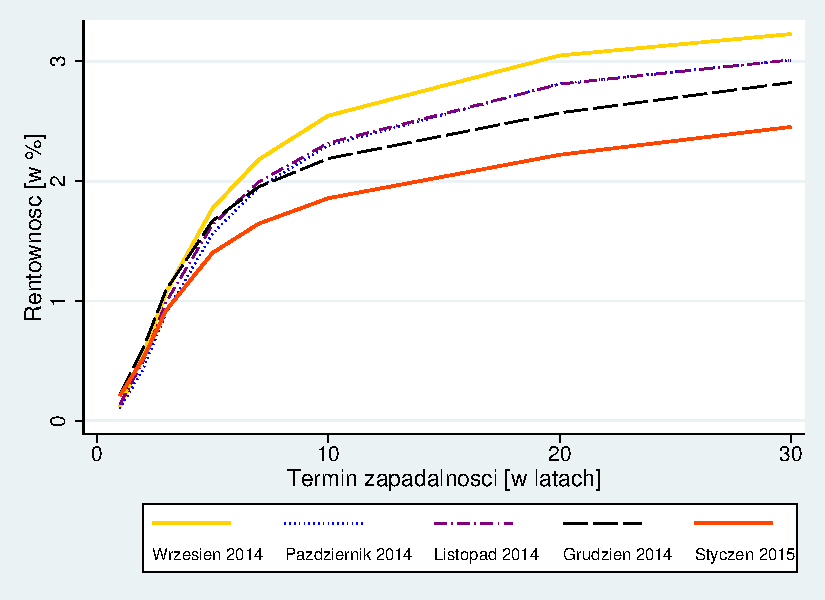
\includegraphics[height=4in]{krzywa10}
    \captionsetup{format=hang}
    \caption{Reakcja krzywej dochodowości na ogłoszenie \protect\hyperlink{kom10}{komunikatu 10} (zakończenie QE3)}
\end{centering}
\begin{flushleft}
\hspace{1cm}\textit{\footnotesize{Źródło: Opracowanie własne.}} \\
\end{flushleft}
\vspace{-0.5cm}
\end{figure}

Pomimo braku istotności \hyperlink{kom10}{komunikatu 10} w~kontekście krótkoterminowego wpływu na średnie dzienne rentowności, istotności tego komunikatu można domniemywać patrząc na dłuższą perspektywę czasową. Na \hyperlink{fig12}{wykresie 11} widać istotną zmianę (około -50~p.b.) rentowności amerykańskich obligacji skarbowych pomiędzy wrześniem 2014~a~styczniem 2015, jednak kierunek tej zmiany jest inny niż można by się spodziewać -  trzy miesiące po zakończeniu bezprecedensowego skupu długoterminowych aktywów krzywa dochodowości osiągnęła na swym dłuższym krańcu niższy poziom niż w~którymkolwiek momencie stosowania niekonwencjonalnej polityki pieniężnej. Mogło to być spowodowane czynnikami zupełnie nie związanymi z~polityką monetarną Rezerwy Federalnej, a~generalnym wzrostem niepewności na rynkach finansowych spowodowanym kolejną odsłoną kryzysu zadłużeniowego w~Grecji i~związaną~z~tym~ucieczką inwestorów do tak zwanych "bezpiecznych przystani"\footnote{Bezpieczna przystań (ang. \textit{safe haven}) to aktywo finansowe, które w~czasie turbulencji na globalnych rynkach finansowych zachowuje swoją wartość, gwarantując inwestorom minimalne ryzyko kosztem minimalnego zysku lub niewielkiej straty}, jakimi niewątpliwie są amerykańskie papiery skarbowe.

Analiza graficzna wykresów miesięcznych krzywych dochodowości nie przynosi jednoznacznych wniosków co do skuteczności decyzji Rezerwy Federalnej w~kształtowaniu krzywej dochodowości amerykańskich obligacji skarbowych. Można zaobserwować wyraźną różnicę pomiędzy reakcją krzywych dochodowości w~najważniejszych momentach stosowania programu pierwszego luzowania ilościowego, a~reakcją w~podobnych momentach dla pozostałych programów - w~przypadku \acs{QE}1 rentowności obligacji zdają się reagować silniej, reakcje te są statystycznie istotne i~są zgodne z~intencją Rezerwy Federalnej. Porównywalne reakcje wywoływały tylko zapowiedzi wskazujące na zakończenie stosowania niekonwencjonalnej polityki monetarnej. W~większości przypadków bezpośrednio po ogłoszeniu komunikatu o~zmianie polityki pieniężnej krzywe dochodowości reagowały wzrostem często wbrew deklarowanym intencjom amerykańskich władz monetarnych i~wzrosty te były następnie kontynuowane w~kolejnych miesiącach\footnote{Opisywane zmiany rentowności długoterminowych obligacji skarbowych Stanów Zjednoczonych są sprzeczne z~wioskami płynącymi z~analizy literatury badawczej przedstawionej w~rozdziale drugim, gdzie stwierdzono statystyczną istotność wpływu niekonwencjonalnej polityki monetarnej na obniżenie rentowności amerykańskich papierów dłużnych.}. O~ile takie zachowanie rynku można by spróbować wytłumaczyć, w~początkowym etapie kryzysu gospodarczego (lata 2008-2009), wyjątkowo wysokim poziomem zmienności rynków finansowych, o tyle po 2009~roku takie wytłumaczenie nie ma racjonalnych przesłanek. Na początku 2010~roku problemy finansowe Grecji rozpoczęły kryzys zadłużeniowy w~strefie euro, amerykańskie obligacje umocniły swoją pozycję jako bezpieczna przystań dla inwestorów, co powinno wywołać presję na wzrost ich cen i~spadek rentowności - w~efekcie wspomagając niekonwencjonalną politykę pieniężną prowadzoną przez Rezerwę Federalną. Nie miało to jednak miejsca - rentowności amerykańskich obligacji skarbowych w~okresie 2010-2Q2016 wahały się w~tunelu [0,25\%; 3-4,5\%] bez wyraźnego trendu. Możliwe więc, iż popyt na rynku dłużnych papierów skarbowych, w~momencie gdy zmalała niepewność związana z~kryzysem w~Stanach Zjednoczonych, został częściowo zniwelowany przez okazje inwestycyjne na innych rynkach finansowych (akcyjnym, nieruchomości, surowcowym) lub też pieniądze z~tego rynku trafiały bezpośrednio do przedsiębiorców realizujących projekty biznesowe i~w ten sposób napędzały amerykańską gospodarkę (co byłoby zgodne z~intencją Rezerwy Federalnej). Wyjaśniałoby to reakcję krzywej dochodowości na ogłaszanie kolejnych niekonwencjonalnych programów po \acs{QE}1 (wzrosty rentowności). Programy te mogły być impulsem do kolejnych odpływów kapitału z~rynków dłużnych papierów wartościowych ku rynkom obarczonym większym ryzykiem. Byłoby to częściowo zgodne z~obserwacjami zawartymi w~literaturze badawczej, gdzie odnotowano wpływ niekonwencjonalnej polityki monetarnej na wzrost cen akcji (\cite{chen36}/\cite{bhattarai36}/\cite{swanson37}). Warto zbadać tę hipotezę sprawdzając wpływ działań amerykańskich władz monetarnych nie tylko na krzywą dochodowości ale także na wskaźniki reprezentujące inne segmenty gospodarki Stanów Zjednoczonych. Tego właśnie dotyczyć będzie następny podrozdział niniejszej pracy.

\hypertarget{podrz32}{}
\phantomsection	% do hiperlinków dla sekcji w spisie treści
\section*{\large{3.2. Skuteczność w~oddziaływaniu na wybrane sektory amerykańskiej gospodarki}}
\addcontentsline{toc}{section}{3.2. Skuteczność w~oddziaływaniu na wybrane sektory amerykańskiej gospodarki}

W~tej części pracy przeprowadzone zostanie badanie empiryczne wpływu niekonwencjonalnej polityki monetarnej Rezerwy Federalnej na amerykańską gospodarkę w~latach 2008-2016. Będzie to próba rozszerzenia badania przeprowadzonego w~poprzedniej części pracy o~zmienne reprezentujące inne segmenty gospodarki Stanów Zjednoczonych niż tylko rynek dłużnych papierów skarbowych. Wydłużony zostanie też horyzont badanego wpływu - w~poprzednim rozdziale był to horyzont od kilkudziesięciu dni (testy istotności) do 5~miesięcy (analiza graficzna kształtu krzywej dochodowości) - w~tym rozdziale horyzontem badawczym będzie rok, czyli średni czas trwania niekonwencjonalnych programów stosowanych przez Rezerwę Federalną. Aby to osiągnąć wykorzystany zostanie model wektorowej autoregresji. W~pierwszej fazie przedstawiony zostanie krótki opis zmiennych wykorzystanych w~badaniu, następnie nakreślona zostanie specyfikacja modelu \acs{VAR} wraz z~jego testami diagnostycznymi, a~na końcu opisane zostaną najważniejsze wnioski wypływające z~modelu, skupiając się w~szczególności na analizie funkcji odpowiedzi na impuls, dekompozycji wariancji prognoz oraz na samych prognozach.

\phantomsection% do hiperlinków dla sekcji w spisie treści
\subsection*{\normalsize{3.2.1. Opis zbioru danych i~specyfikacja modelu}}
\addcontentsline{toc}{subsection}{3.2.1. Opis zbioru danych i~specyfikacja modelu}
\vspace{0.4cm}

Konstrukcję modelu wektorowej autoregresji rozpoczęto od stworzenia wstępnej bazy 32~zmiennych reprezentujących wybrane segmenty gospodarki Stanów Zjednoczonych. Ich wybór wynikał bezpośrednio z~analizy literatury dotyczącej niekonwencjonalnej polityki pieniężnej stosowanej przez bank Rezerwy Federalnej w~latach 2008-2016, przeprowadzonej w~drugim rozdziale niniejszej pracy. Każda ze zmiennych składa się z~174~miesięcznych obserwacji z~lat 2002-2016, przy czym w~końcowym modelu \acs{VAR} wykorzystano tylko 96~ostatnich obserwacji (z~okresu lipiec 2008 - czerwiec 2016), gdyż to właśnie na tym okresie, zgodnie z~literaturą badawczą, postanowiono się skupić (dane z~wcześniejszych lat zostały wykorzystane przy badaniu wstecznej jakości prognoz finalnego modelu). Ośmioletnia szerokość próbki złożona wyłącznie z~obserwacji następujących po wybuchu kryzysu finansowego oraz zastosowanie częstotliwości miesięcznej poskutkowało uzyskaniem 96~unikalnych, nieinterpolowanych obserwacji, co jest elementem wyróżniającymi badanie przedstawione w~niniejszej pracy spośród innych dostępnych opracowań dotyczących niekonwencjonalnej polityki pieniężnej. Oparcie modelu \acs{VAR} na danych miesięcznych i~skrócenie próby do lat 2008-2016 miało na celu uchwycenie relacji pomiędzy zmiennymi w~krótkoterminowej perspektywie (do roku), gwarancję satysfakcjonującej liczby stopni swobody oraz skupienie analizy na spójnym badawczo okresie - wybuch kryzysu finansowego w~2008~roku spowodował na tyle istotne zmiany makroekonomiczne w~gospodarce Stanów Zjednoczonych, iż niewskazane byłoby uwzględnianie w~modelu obserwacji, które nie były poddane tym zmianom (obserwacje przed wybuchem kryzysu). \hyperlink{zal1}{Załącznik 1} prezentuje podsumowanie najważniejszych informacji dotyczących zmiennych wybranych do wstępnej analizy pod kątem zastosowania ich w~finalnym modelu wektorowej autoregresji. Źródłem pozyskania większości z~nich jest strona internetowa Banku Rezerwy Federalnej w~Saint Louis (\url{http://research.stlouisfed.org}) poza zmienną \textit{PKB_realne}, która została pozyskana ze strony internetowej Macroeconomic Advisers LLC (\url{http://www.macroadvisers.com/}) ze względu na brak dostępności tej zmiennej w~częstotliwości miesięcznej na stronach internetowych FED.

Po wstępnym wyborze zmiennych i~uzyskaniu ich miesięcznych obserwacji postanowiono przyjrzeć się ich podstawowym statystykom opisowym oraz wykresom. Na tej podstawie zdecydowano się dokonać transformacji logarytmicznej części z~nich ze względu na ich wykładniczy wzrost (\textit{Zatrudnienie} i~\textit{Kred_bank}). Następnie przeprowadzono testy na stacjonarność w~okresie badawczym (2008-2016), aby określić stopień zintegrowania każdej z~nich, bardzo ważny pod kątem właściwej specyfikacji modelu wektorowej autoregresji. Od poziomu zintegrowania zmiennych w~modelu zależy możliwość interpretacji jego oszacowania bez obaw o~występowanie problemu regresji pozornej. Większość zmiennych okazała się zintegrowana w~stopniu 1 (21 spośród 32), sześć zmiennych było zintegrowanych w~stopniu 2~oraz pięć zmiennych zidentyfikowano jako stacjonarne (zintegrowane w~stopniu 0) - patrz \hyperlink{zal1}{załącznik 1}. Po analizie zarówno pod kątem literatury badawczej (rozdział 2), reprezentatywności segmentów gospodarki, konstrukcji modelu, jego jakości dopasowania do danych, stabilności oraz złożoności, zdecydowano się do finalnego modelu VAR wykorzystać następujące 9~zmiennych, gwarantujących jego najwyższą jakość badawczą: 
\begin{itemize}
\setlength\itemsep{0.05cm}
\item Indeks prywatnych wydatków konsumpcyjnych (poziom cen),
\item Stopa bezrobocia (rynek pracy),
\item Roczna zmiana \acs{PKB} realnego (poziom produkcji),
\item Indeks S\&P500 (rynek akcji),
\item Rentowność rocznych obligacji skarbowych (rynek obligacji skarbowych),
\item Rentowność dziesięcioletnich obligacji skarbowych (rynek obligacji skarbowych),
\item Wartość papierów wartościowych w~bilansie Rezerwy Federalnej  (poziom cen),
\item Mediana czasu trwania bezrobocia (rynku pracy),
\item Kurs walutowy EUR/USD (rynek walutowy).
\end{itemize}

\noindent Zmienne wybrane do finalnego modelu \acs{VAR} reprezentują segmenty amerykańskiej gospodarki, na które bank centralny Stanów Zjednoczonych mógł bezpośrednio lub pośrednio wpływać stosując niekonwencjonalną politykę monetarną. Tymi segmentami są: rynek pracy, rynek walutowy, rynek akcji, poziom cen, poziom produkcji oraz poddany szczegółowej analizie w~poprzednim podrozdziale rynek obligacji skarbowych. Finalne zmienne mają różne poziomy zintegrowania, w~większości nie są to zmienne stacjonarne - w~związku z~tym analizie poddane zostaną zatem wyłącznie relacje występujące pomiędzy zmiennymi reprezentowane przez funkcje odpowiedzi na impuls, dekompozycja wariancji błędów prognoz oraz prognozy uzyskane z~modelu.

\vspace{0.25cm}
\hypertarget{tab4}{}
\begin{table}[!ht]
\rowcolors{3}{white}{lightgray}
\captionsetup{format=hang, position=top}
\caption{Kryteria informacyjne - sugerowana liczba opóźnień w~modelu VAR}
\begin{tabular}{
M{7.5cm}
S[table-format=3.4]
M{3cm}
}
\toprule
\textbf{Nazwa} & \textbf{Minimalna wartość} & \textbf{Liczba opóźnień}\\
\textbf{kryterium} &  {\textbf{kryterium}} & \textbf{w modelu VAR}\\
\midrule
Kryterium informacyjne Akaikego & -1,1495  &       6 \\
Kryterium informacyjne Hannana–Quinna & 2,8061 &      2 \\
Kryterium Schwarza  &    4,7751      &       1 \\
Ostateczny błąd predykcji Akaikego & 1,4417  &       4 \\
\bottomrule
\end{tabular}
\begin{flushleft}
\hspace{1cm}\textit{\footnotesize{Źródło: Opracowanie własne.}} \\
\end{flushleft}
\vspace{-0.5cm}
\end{table} 

Kolejnym etapem konstrukcji finalnego modelu \acs{VAR} był wybór odpowiedniej liczby opóźnień zmiennych endogenicznych, w~tym celu posłużono się czterema najczęściej stosowanymi w~literaturze testami opartymi o~minimalizację kryteriów informacyjnych: \acs{AIC}, \acs{HQIC}, \acs{SC} i \acs{AFPE}. Założono przy tym, iż maksymalna liczba opóźnień nie może przekroczyć sześciu - większa liczba mogłaby spowodować zbyt duże ograniczenie stopni swobody. \hyperlink{tab4}{Tabela 5} prezentuje sugerowaną optymalną liczbę opóźnień w~modelu \acs{VAR} wyznaczoną na podstawie minimalizacji odpowiedniego kryterium informacyjnego. W~związku z~tym, iż każde z~kryteriów wskazuje na inną liczbę opóźnień, zdecydowano się wybrać model z~trzema opóźnieniami, gdyż model z~taką liczbą opóźnień gwarantuje drugą najniższą łączną wartość kryteriów informacyjnych przy najlepszych wynikach testów diagnostycznych. Po wyborze zmiennych oraz po określeniu optymalnej liczby opóźnień możliwe stało się przedstawienie zapisu matematycznego finalnego modelu wektorowej autoregresji, z~którego będziemy korzystać w~niniejszej pracy - przedstawia go \hyperlink{row22}{równanie 8}. 

\vspace{-0.5cm}
\hypertarget{row22}{}
\scriptsize
\begin{equation}
\begin{aligned}
Y =
\begin{bmatrix}
       PCE_{t} \\[0.05em]
       Stopa\_bez_{ t} \\[0.05em]
       PKB\_realne_{t} \\[0.05em]
       SP500_{t} \\[0.05em]
       Yield10Gov_{t} \\[0.05em]
       Yield1YGov_{t} \\[0.05em]
       FED\_Securities_{t} \\[0.05em]
       UnempDur_{t} \\[0.05em]
       EURUSD_{t} 
\end{bmatrix} ={} &
\begin{bmatrix}
       c_1 \\[0.05em]
       c_2 \\[0.05em]
       c_3 \\[0.05em]
       c_4 \\[0.05em]
       c_5 \\[0.05em]
       c_6 \\[0.05em]
       c_7 \\[0.05em]
       c_8 \\[0.05em]
       c_9
\end{bmatrix} +
\begin{bmatrix}
\beta^1_{1,1} & \beta^1_{1,2} & \beta^1_{1,3} & \beta^1_{1,4} & \beta^1_{1,5} & \beta^1_{1,6} & \beta^1_{1,7} & \beta^1_{1,8} &   \beta^1_{1,9} \\[0.05em]
\beta^1_{2,1} & \beta^1_{2,2} & \beta^1_{2,3} & \beta^1_{2,4} & \beta^1_{2,5} & \beta^1_{2,6} & \beta^1_{2,7} & \beta^1_{2,8} &   \beta^1_{2,9} \\[0.05em]
\beta^1_{3,1} & \beta^1_{3,2} & \beta^1_{3,3} & \beta^1_{3,4} & \beta^1_{3,5} & \beta^1_{3,6} & \beta^1_{3,7} & \beta^1_{3,8} &   \beta^1_{3,9} \\[0.05em]
\beta^1_{4,1} & \beta^1_{4,2} & \beta^1_{4,3} & \beta^1_{4,4} & \beta^1_{4,5} & \beta^1_{4,6} & \beta^1_{4,7} & \beta^1_{4,8} &   \beta^1_{4,9} \\[0.05em]
\beta^1_{5,1} & \beta^1_{5,2} & \beta^1_{5,3} & \beta^1_{5,4} & \beta^1_{5,5} & \beta^1_{5,6} & \beta^1_{5,7} & \beta^1_{5,8} &   \beta^1_{5,9} \\[0.05em]
\beta^1_{6,1} & \beta^1_{6,2} & \beta^1_{6,3} & \beta^1_{6,4} & \beta^1_{6,5} & \beta^1_{6,6} & \beta^1_{6,7} & \beta^1_{6,8} &   \beta^1_{6,9} \\[0.05em]
\beta^1_{7,1} & \beta^1_{7,2} & \beta^1_{7,3} & \beta^1_{7,4} & \beta^1_{7,5} & \beta^1_{7,6} & \beta^1_{7,7} & \beta^1_{7,8} &   \beta^1_{7,9} \\[0.05em]
\beta^1_{8,1} & \beta^1_{8,2} & \beta^1_{8,3} & \beta^1_{8,4} & \beta^1_{8,5} & \beta^1_{8,6} & \beta^1_{8,7} & \beta^1_{8,8} &   \beta^1_{8,9} \\[0.05em]
\beta^1_{9,1} & \beta^1_{9,2} & \beta^1_{9,3} & \beta^1_{9,4} & \beta^1_{9,5} & \beta^1_{9,6} & \beta^1_{9,7} & \beta^1_{9,8} &   \beta^1_{9,9}
\end{bmatrix}
\begin{bmatrix}
       PCE_{t-1} \\[0.05em]
       Stopa\_bez_{ t-1} \\[0.05em]
       PKB\_realne_{t-1} \\[0.05em]
       SP500_{t-1} \\[0.05em]
       Yield10Gov_{t-1} \\[0.05em]
       Yield1YGov_{t-1} \\[0.05em]
       FED\_Securities_{t-1} \\[0.05em]
       UnempDur_{t-1} \\[0.05em]
       EURUSD_{t-1} 
\end{bmatrix} + \\ &
\begin{bmatrix}
\beta^2_{1,1} & \beta^2_{1,2} & \beta^2_{1,3} & \beta^2_{1,4} & \beta^2_{1,5} & \beta^2_{1,6} & \beta^2_{1,7} & \beta^2_{1,8} &   \beta^2_{1,9} \\[0.05em]
\beta^2_{2,1} & \beta^2_{2,2} & \beta^2_{2,3} & \beta^2_{2,4} & \beta^2_{2,5} & \beta^2_{2,6} & \beta^2_{2,7} & \beta^2_{2,8} &   \beta^2_{2,9} \\[0.05em]
\beta^2_{3,1} & \beta^2_{3,2} & \beta^2_{3,3} & \beta^2_{3,4} & \beta^2_{3,5} & \beta^2_{3,6} & \beta^2_{3,7} & \beta^2_{3,8} &   \beta^2_{3,9} \\[0.05em]
\beta^2_{4,1} & \beta^2_{4,2} & \beta^2_{4,3} & \beta^2_{4,4} & \beta^2_{4,5} & \beta^2_{4,6} & \beta^2_{4,7} & \beta^2_{4,8} &   \beta^2_{4,9} \\[0.05em]
\beta^2_{5,1} & \beta^2_{5,2} & \beta^2_{5,3} & \beta^2_{5,4} & \beta^2_{5,5} & \beta^2_{5,6} & \beta^2_{5,7} & \beta^2_{5,8} &   \beta^2_{5,9} \\[0.05em]
\beta^2_{6,1} & \beta^2_{6,2} & \beta^2_{6,3} & \beta^2_{6,4} & \beta^2_{6,5} & \beta^2_{6,6} & \beta^2_{6,7} & \beta^2_{6,8} &   \beta^2_{6,9} \\[0.05em]
\beta^2_{7,1} & \beta^2_{7,2} & \beta^2_{7,3} & \beta^2_{7,4} & \beta^2_{7,5} & \beta^2_{7,6} & \beta^2_{7,7} & \beta^2_{7,8} &   \beta^2_{7,9} \\[0.05em]
\beta^2_{8,1} & \beta^2_{8,2} & \beta^2_{8,3} & \beta^2_{8,4} & \beta^2_{8,5} & \beta^2_{8,6} & \beta^2_{8,7} & \beta^2_{8,8} &   \beta^2_{8,9} \\[0.05em]
\beta^2_{9,1} & \beta^2_{9,2} & \beta^2_{9,3} & \beta^2_{9,4} & \beta^2_{9,5} & \beta^2_{9,6} & \beta^2_{9,7} & \beta^2_{9,8} &   \beta^2_{9,9}
\end{bmatrix}
\begin{bmatrix}
       PCE_{t-2} \\[0.05em]
       Stopa\_bez_{ t-2} \\[0.05em]
       PKB\_realne_{t-2} \\[0.05em]
       SP500_{t-2} \\[0.05em]
       Yield10Gov_{t-2} \\[0.05em]
       Yield1YGov_{t-2} \\[0.05em]
       FED\_Securities_{t-2} \\[0.05em]
       UnempDur_{t-2} \\[0.05em]
       EURUSD_{t-2} 
\end{bmatrix} + \\ &
\begin{bmatrix}
\beta^3_{1,1} & \beta^3_{1,2} & \beta^3_{1,3} & \beta^3_{1,4} & \beta^3_{1,5} & \beta^3_{1,6} & \beta^3_{1,7} & \beta^3_{1,8} &   \beta^3_{1,9} \\[0.05em]
\beta^3_{2,1} & \beta^3_{2,2} & \beta^3_{2,3} & \beta^3_{2,4} & \beta^3_{2,5} & \beta^3_{2,6} & \beta^3_{2,7} & \beta^3_{2,8} &   \beta^3_{2,9} \\[0.05em]
\beta^3_{3,1} & \beta^3_{3,2} & \beta^3_{3,3} & \beta^3_{3,4} & \beta^3_{3,5} & \beta^3_{3,6} & \beta^3_{3,7} & \beta^3_{3,8} &   \beta^3_{3,9} \\[0.05em]
\beta^3_{4,1} & \beta^3_{4,2} & \beta^3_{4,3} & \beta^3_{4,4} & \beta^3_{4,5} & \beta^3_{4,6} & \beta^3_{4,7} & \beta^3_{4,8} &   \beta^3_{4,9} \\[0.05em]
\beta^3_{5,1} & \beta^3_{5,2} & \beta^3_{5,3} & \beta^3_{5,4} & \beta^3_{5,5} & \beta^3_{5,6} & \beta^3_{5,7} & \beta^3_{5,8} &   \beta^3_{5,9} \\[0.05em]
\beta^3_{6,1} & \beta^3_{6,2} & \beta^3_{6,3} & \beta^3_{6,4} & \beta^3_{6,5} & \beta^3_{6,6} & \beta^3_{6,7} & \beta^3_{6,8} &   \beta^3_{6,9} \\[0.05em]
\beta^3_{7,1} & \beta^3_{7,2} & \beta^3_{7,3} & \beta^3_{7,4} & \beta^3_{7,5} & \beta^3_{7,6} & \beta^3_{7,7} & \beta^3_{7,8} &   \beta^3_{7,9} \\[0.05em]
\beta^3_{8,1} & \beta^3_{8,2} & \beta^3_{8,3} & \beta^3_{8,4} & \beta^3_{8,5} & \beta^3_{8,6} & \beta^3_{8,7} & \beta^3_{8,8} &   \beta^3_{8,9} \\[0.05em]
\beta^3_{9,1} & \beta^3_{9,2} & \beta^3_{9,3} & \beta^3_{9,4} & \beta^3_{9,5} & \beta^3_{9,6} & \beta^3_{9,7} & \beta^3_{9,8} &   \beta^3_{9,9}
\end{bmatrix}
\begin{bmatrix}
       PCE_{t-3} \\[0.05em]
       Stopa\_bez_{t-3} \\[0.05em]
       PKB\_realne_{t-3} \\[0.05em]
       SP500_{t-3} \\[0.05em]
       Yield10Gov_{t-3} \\[0.05em]
       Yield1YGov_{t-3} \\[0.05em]
       FED\_Securities_{t-3} \\[0.05em]
       UnempDur_{t-3} \\[0.05em]
       EURUSD_{t-3} 
\end{bmatrix} +
\begin{bmatrix}
       \epsilon_{1,t}  \\[0.05em]
       \epsilon_{2,t}  \\[0.05em]
       \epsilon_{3,t}  \\[0.05em]
       \epsilon_{4,t}  \\[0.05em]
       \epsilon_{5,t}  \\[0.05em]
       \epsilon_{6,t}  \\[0.05em]
       \epsilon_{7,t}  \\[0.05em] 
       \epsilon_{8,t}  \\[0.05em]
       \epsilon_{9,t}  
\end{bmatrix}
\end{aligned}
\end{equation}
\normalsize

\noindent Jak wskazuje powyższy zapis \hyperlink{row22}{równania}, w~finalnym modelu oszacowanych zostanie 252 parametrów - 243 współczynniki $\beta$ oraz 9~stałych. \hyperlink{zal2}{Załącznik 2} prezentuje wykresy dopasowań zmiennych oraz reszt w~finalnym modelu \acs{VAR}. Analiza tych wykresów wskazuje na dobre dopasowanie zmiennych, stabilność modelu oraz właściwe rozkłady reszt. Warto potwierdzić te wnioski stosując testy diagnostyczne - zbadana zostanie przede wszystkim stabilność strukturalna modelu, normalność składnika losowego oraz obecność autokorelacji lub homoskedastycznosci wśród reszt (sferyczność błędu losowego). \hyperlink{tab5}{Tabela 6} prezentuje wyniki zastosowanych testów diagnostycznych. 

\hypertarget{tab5}{}
\begin{table}[!ht]
\rowcolors{2}{lightgray}{white}
\captionsetup{format=hang, position=top}
\caption{Wyniki testów diagnostycznych dla finalnego modelu VAR}
\begin{tabular}{
M{3cm}
M{4cm}
S[table-format=4.1]
S[table-format=1.4]
}
\toprule
\textbf{Nazwa testu} & \textbf{Hipoteza zerowa} & \textbf{St. testowa} & \textbf{P-value} \\
\midrule
Test Portmanteau &  Brak autokorelacji  &  1132,1 &  0,0449 \\
Test Jarque-Berra &   Normalność reszt   &  24,6  &  0,1368 \\
Test skośności  &   Normalność reszt   &  12,7 &  0,1772 \\
Test kurtozy   &   Normalność reszt   &  11,9  &  0,2192 \\
Test ARCH-LM  & Heteroskedastyczność &  4050,0  &  1,0000 \\
\bottomrule
\end{tabular}
\begin{flushleft}
\hspace{1cm}\textit{\footnotesize{Źródło: Opracowanie własne.}} \\
\end{flushleft}
\vspace{-0.5cm}
\end{table} 

Wynik testu Portmanteau na obecność autokorelacji reszt w~modelu przypada na granicy pomiędzy 4\%-owym, a~5\%-owym poziomem istotności (stosowanym jako bazowy w~niniejszej pracy). W~związku z~tym, iż zmiana poziomu istotności do 4\%, prowadzi do większej rygorystyczności testu diagnostycznego, można dokonać takiej zmiany na potrzeby tego testu i~stwierdzić brak konieczności odrzucenia hipotezy zerowej o~braku autokorelacji. Jedno z~podstawowych założeń modelu \acs{VAR} zostało więc spełnione. Podobnie testy na normalność wskazują, iż nie ma podstaw do odrzucenia hipotez zerowych o~normalności składnika losowego w~modelu - co oznacza spełnienie kolejnego podstawowego założenia modelu. W~przypadku testu ARCH-LM wynik okazał się niezadowalający - w modelu występuje problem heteroskedastyczności, który może obciążać oszacowania parametrów finalnego modelu VAR, jednak nie wpłynie na zniekształcenie wniosków płynących z~analizy zależności pomiędzy zmiennymi. Można było się spodziewać takiego wyniku testu ARCH-LM ze względu na fakt, iż większość danych finansowych obciążonych jest problemem heteroskedastyczności reszt w~związku ze swoją relatywnie wysoką zmiennością (szczególnie w~okresach kryzysu). Już na etapie wyboru zmiennych założono, iż celem badania nie będzie interpretacja oszacowań parametrów modelu tylko analiza relacji występujących pomiędzy zmiennymi stąd heteroskedastycność wśród reszt nie będzie przeszkodą w~kontynuowaniu badania.

Ostatnim, niezaprezentowanym w~\hyperlink{tab5}{tabeli 6} testem badającym jakość modelu wektorowej autoregresji jest test na jego strukturalną stabilność. Aby go wykonać należy wyznaczyć wektor wartości własnych macierzy stowarzyszonej współczynników modelu i~sprawdzić czy każdy element takiego wektora jest mniejszy od jedności - co oznacza, iż w~modelu brak jest pierwiastka jednostkowego. W~przypadku finalnego modelu wektorowej autoregresji, omawianego w~tym rozdziale, otrzymano wektor wartości własnych z~maksymalnym elementem równym 0,9475~co wskazuje, iż model ten jest strukturalnie stabilny - można przy jego pomocy generować efektywne prognozy i~analizować relacje pomiędzy zmiennymi. Po ukończeniu procedury selekcji danych, konstrukcji modelu oraz sprawdzenia jego jakości można przejść do etapu wyciągania wniosków i~weryfikacji hipotez badawczych. Analiza ta zostanie oparta na badaniu relacji pomiędzy zmiennymi ukazanych za pomocą funkcji odpowiedzi na impuls, prognoz wartości zmiennych w~przyszłych okresach oraz dekompozycji wariancji błędów tych prognoz.
 
\phantomsection % do hiperlinków dla sekcji w spisie treści
\subsection*{\normalsize{3.2.2. Analiza wyników i~weryfikacja hipotez badawczych}}
\addcontentsline{toc}{subsection}{3.2.2. Analiza wyników i~weryfikacja hipotez badawczych}
\vspace{0.4cm}

Chcąc zbadać wpływ niekonwencjonalnej polityki pieniężnej amerykańskich władz monetarnych na gospodarkę Stanów Zjednoczonych postanowiono skupić się na zbadaniu wpływu zmiennej obrazującej wartość papierów wartościowych w~bilansie Rezerwy Federalnej (zmienna \textit{FED_Securities}) na pozostałe zmienne wykorzystane w~finalnym modelu wektorowej autoregresji. 

\hypertarget{fig13}{}
\begin{figure}[h]
\begin{centering}
  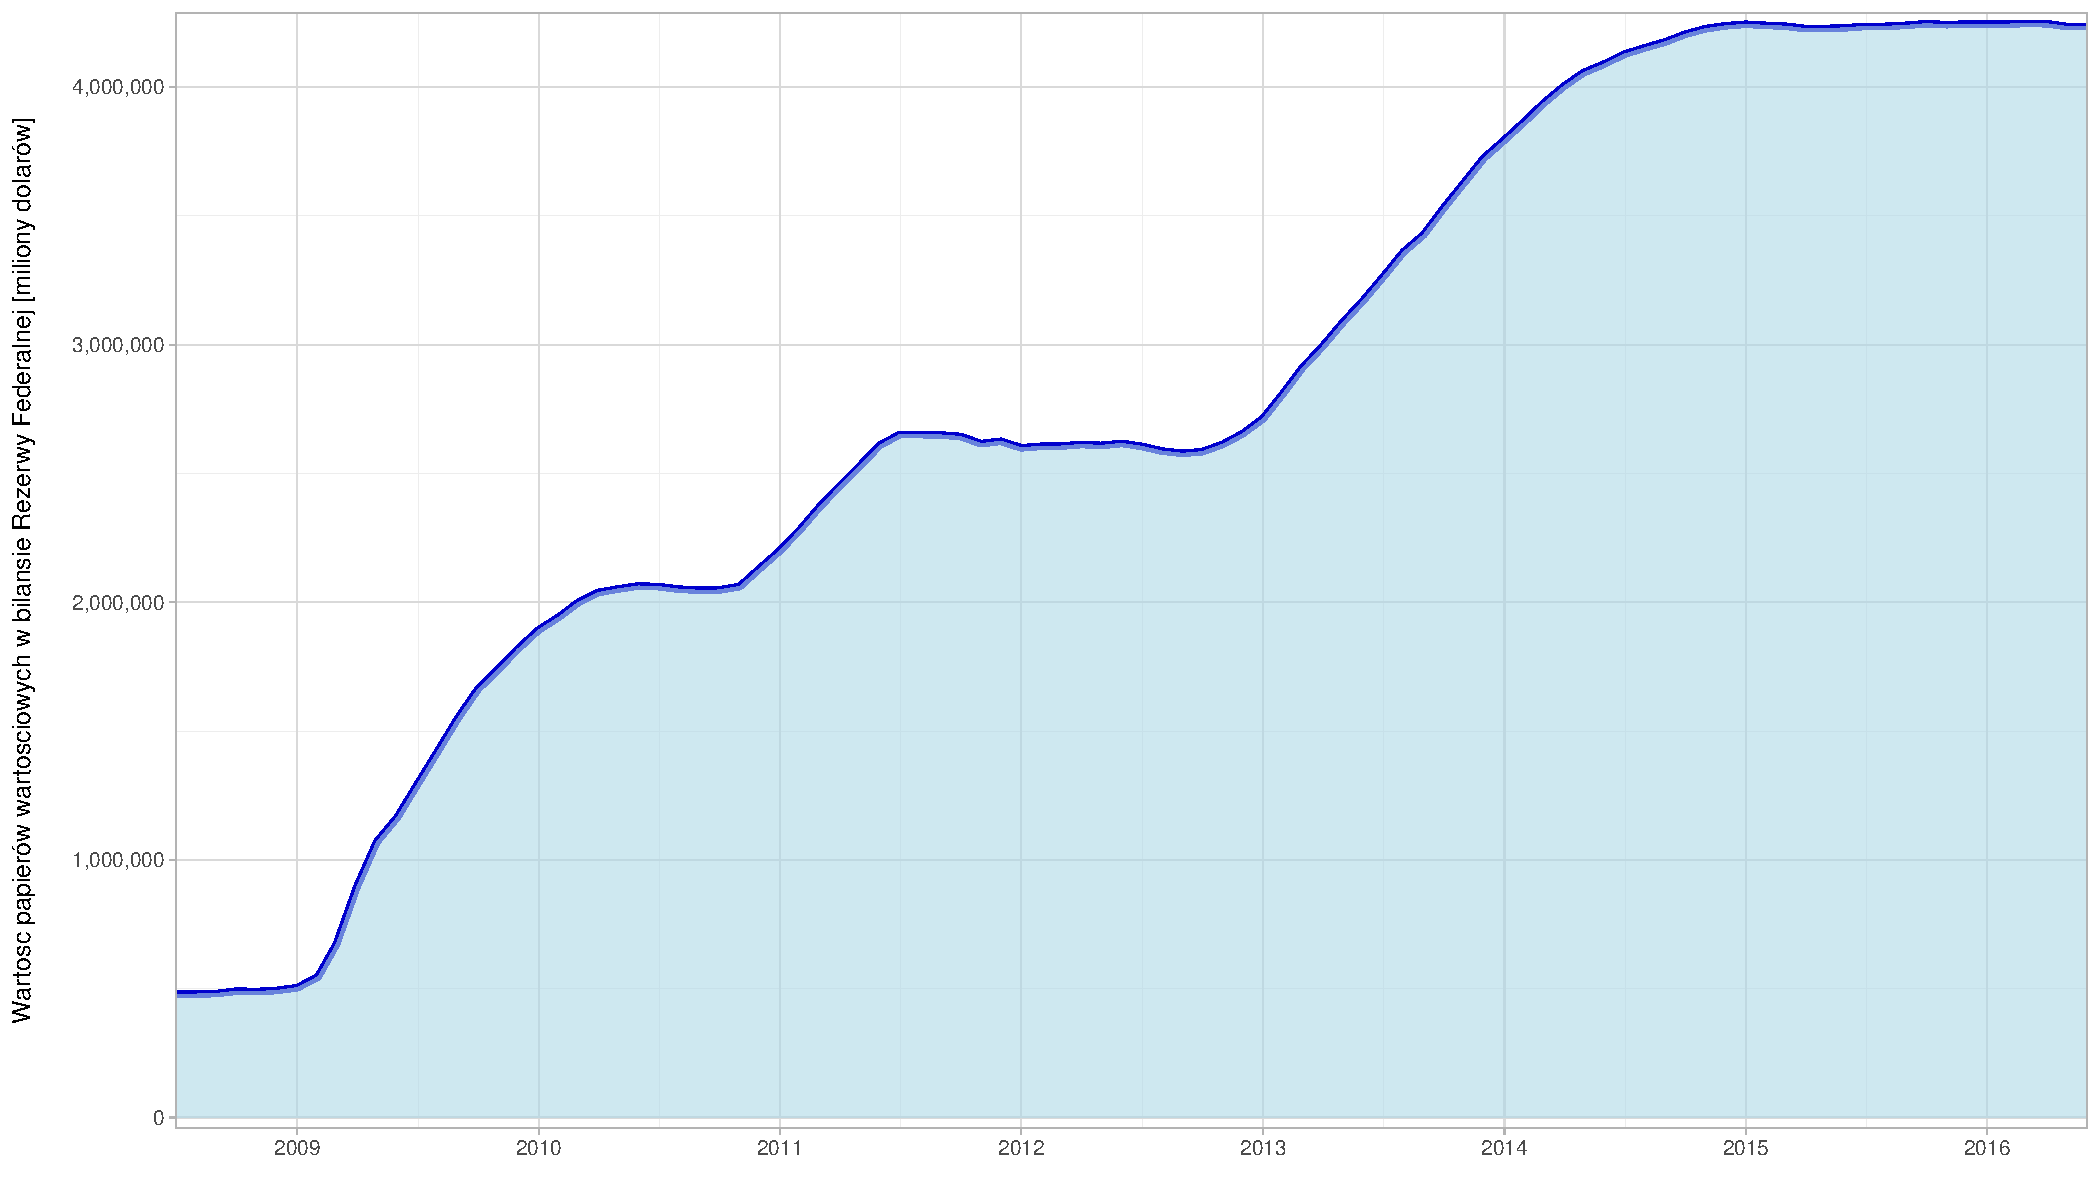
\includegraphics[height=3.5in]{FEDSec}
    \captionsetup{format=hang}
    \caption{Zmienna \textit{FED_Securities} w~okresie 07.2008-06.2016}
\end{centering}
\begin{flushleft}
\hspace{1cm}\textit{\footnotesize{Źródło: Opracowanie własne.}} \\
\end{flushleft}
\vspace{-0.5cm}
\end{figure}

Zmienna \textit{FED_Securities} w~bezpośredni sposób obrazuje skalę i~tempo niekonwencjonalnych działań amerykańskich władz monetarnych na rynkach dłużnych papierów wartościowych (skarbowym i~papierów komercyjnym) w~latach 2008-2016 będąc skumulowaną sumą wartości wszystkich zakupionych przez Rezerwę Federalną papierów wartościowych w~kolejnych odcinkach czasu. \hyperlink{fig13}{Wykres 12} prezentuje sposób w~jaki kształtowała się wyżej wspomniana zmienna w~poszczególnych latach okresu badawczego - widać jej dynamiczny wzrost od końca 2008~roku, z~blisko 500~miliardów dolarów do około 4,5~biliona dolarów, co oznacza przyrost o~niemal 800\% w~6~lat. Tak znacząca kwota pieniędzy (około 25\% \acs{PKB} Stanów Zjednoczonych) wprowadzona przez Rezerwę Federalną na~rynek dłużnych papierów wartościowych w~latach 2008-2016 powinna istotnie wpłynąć na ten segment amerykańskiej gospodarki, ale również nie powinna mieć neutralnego wpływu na pozostałe jej segmenty reprezentowane przez zmienne wykorzystane w~finalnym modelu wektorowej autoregresji. Aby określić czy ten wpływ był statystycznie istotny postanowiono zbadać czy zmienna \textit{FED_Securities} jest przyczyną w~sensie Grangera pozostałych zmiennych. Oznacza to zbadanie, czy przeszłe wartości zmiennej reprezentującej wartość papierów wartościowych w~bilansie Rezerwy Federalnej są w~stanie poprawić jakość prognoz pozostałych zmiennych zawartych w~modelu. W~literaturze często stosuje się również tak zwaną przyczynowość natychmiastową (ang. \textit{instantaneous causality}), która stanowi rozszerzenie przyczynowości w~sensie Grangera o~bieżące wartości badanej zmiennej. Do zbadania czy zmienna \textit{FED_Security} mogła spowodować istotne zmiany pozostałych zmiennych wykorzystanych w~analizowanym w~tym rozdziale modelu postanowiono skorzystać z~obu tych przyczynowości. Do zbadania przyczynowości w~sensie Grangera, jak i~przyczynowości natychmiastowej zastosowano odpowiednie testy statystyczne, których wyniki zaprezentowano w~\hyperlink{tab6}{tabeli nr 7}. 

\hypertarget{tab6}{}
\begin{table}[!ht]
\rowcolors{2}{lightgray}{white}
\captionsetup{format=hang, position=top}
\caption{Wyniki testów na przyczynowość w~sensie Grangera oraz na przyczynowość natychmiastową zmiennej \textit{FED_Securities} w~finalnym modelu VAR}
\begin{tabular}{
M{4.5cm}
M{4cm}
S[table-format=2.3]
S[table-format=1.3]
}
\toprule
\textbf{Nazwa testu} & \textbf{Hipoteza zerowa} & \textbf{St. testowa} & \textbf{P-value} \\
\midrule
Przycz. Granger    &  Brak przyczynowości &   3,862  & 0,000\\
Przycz. natychmiastowa &  Brak przyczynowości &  19,177  & 0.014\\
\bottomrule
\end{tabular}
\begin{flushleft}
\hspace{1cm}\textit{\footnotesize{Źródło: Opracowanie własne.}} \\
\end{flushleft}
\vspace{-0.5cm}
\end{table} 

Wyniki obu testów wskazują, iż na 5\%-owym poziomie istotności należy odrzucić hipotezę zerową o~braku przyczynowości - zmienna \textit{FED_Securities} jest przyczyną zarówno w~sensie Grangera, jak i~natychmiastową, pozostałych zmiennych z~finalnego modelu \acs{VAR}. Oznacza to, iż zasadne jest badanie wpływu niekonwencjonalnej polityki monetarnej Rezerwy Federalnej na zmienne reprezentujące wybrane segmenty amerykańskiej gospodarki.

\subsection*{\normalsize{Analiza funkcji odpowiedzi na impuls finalnego modelu VAR}}

Pierwszym etapem badania relacji pomiędzy zmiennymi w~finalnym modelu \acs{VAR} jest analiza funkcji odpowiedzi na impuls (\acs{IRF}). W~związku z~tym, iż niniejsza praca skupia się na wpływie niekonwencjonalnej polityki pieniężnej na amerykańską gospodarkę, analiza funkcji \acs{IRF} dotyczyć będzie szoku zmiennej \textit{FED_Securities}, zdefiniowanego jako jej jeden błąd standardowy z~badanej próby z~lat 2008-2016 (około 120~miliardów dolarów) oraz jej wpływie na pozostałe zmienne modelu: \textit{PCE}, \textit{Stopa_bez}, \textit{PKB_realne}, \textit{SP500}, \textit{Yield1YGov}, \textit{Yield10Gov}, \textit{UnempDur}, \textit{EURUSD}. \hyperlink{fig14}{Wykres 13}~prezentuje funkcje odpowiedzi na impuls zmiennych finalnego modelu \acs{VAR} oraz odpowiednie 95\%-owe przedziały ufności tych funkcji wyznaczone za pomocą metody \textit{bootstrap} \footnote{Uzyskane przedziały ufności okazały się stosunkowo szerokie. Przedziały podobnej szerokości obserwuje się również w~literaturze dotyczącej niekonwencjonalnej polityki monetarnej i~jest to związane z~niską liczbą stopni swobody wynikającą z~małej liczby obserwacji w~odniesieniu do liczby zmiennych i~ich opóźnień w~modelu}. Ze względu na miesięczną częstotliwość danych zdecydowano się na analizę funkcji \acs{IRF} w~skumulowanej perspektywie rocznej.

\vspace{0.25cm}
\hypertarget{fig14}{}
\begin{figure}[h]
\begin{centering}
  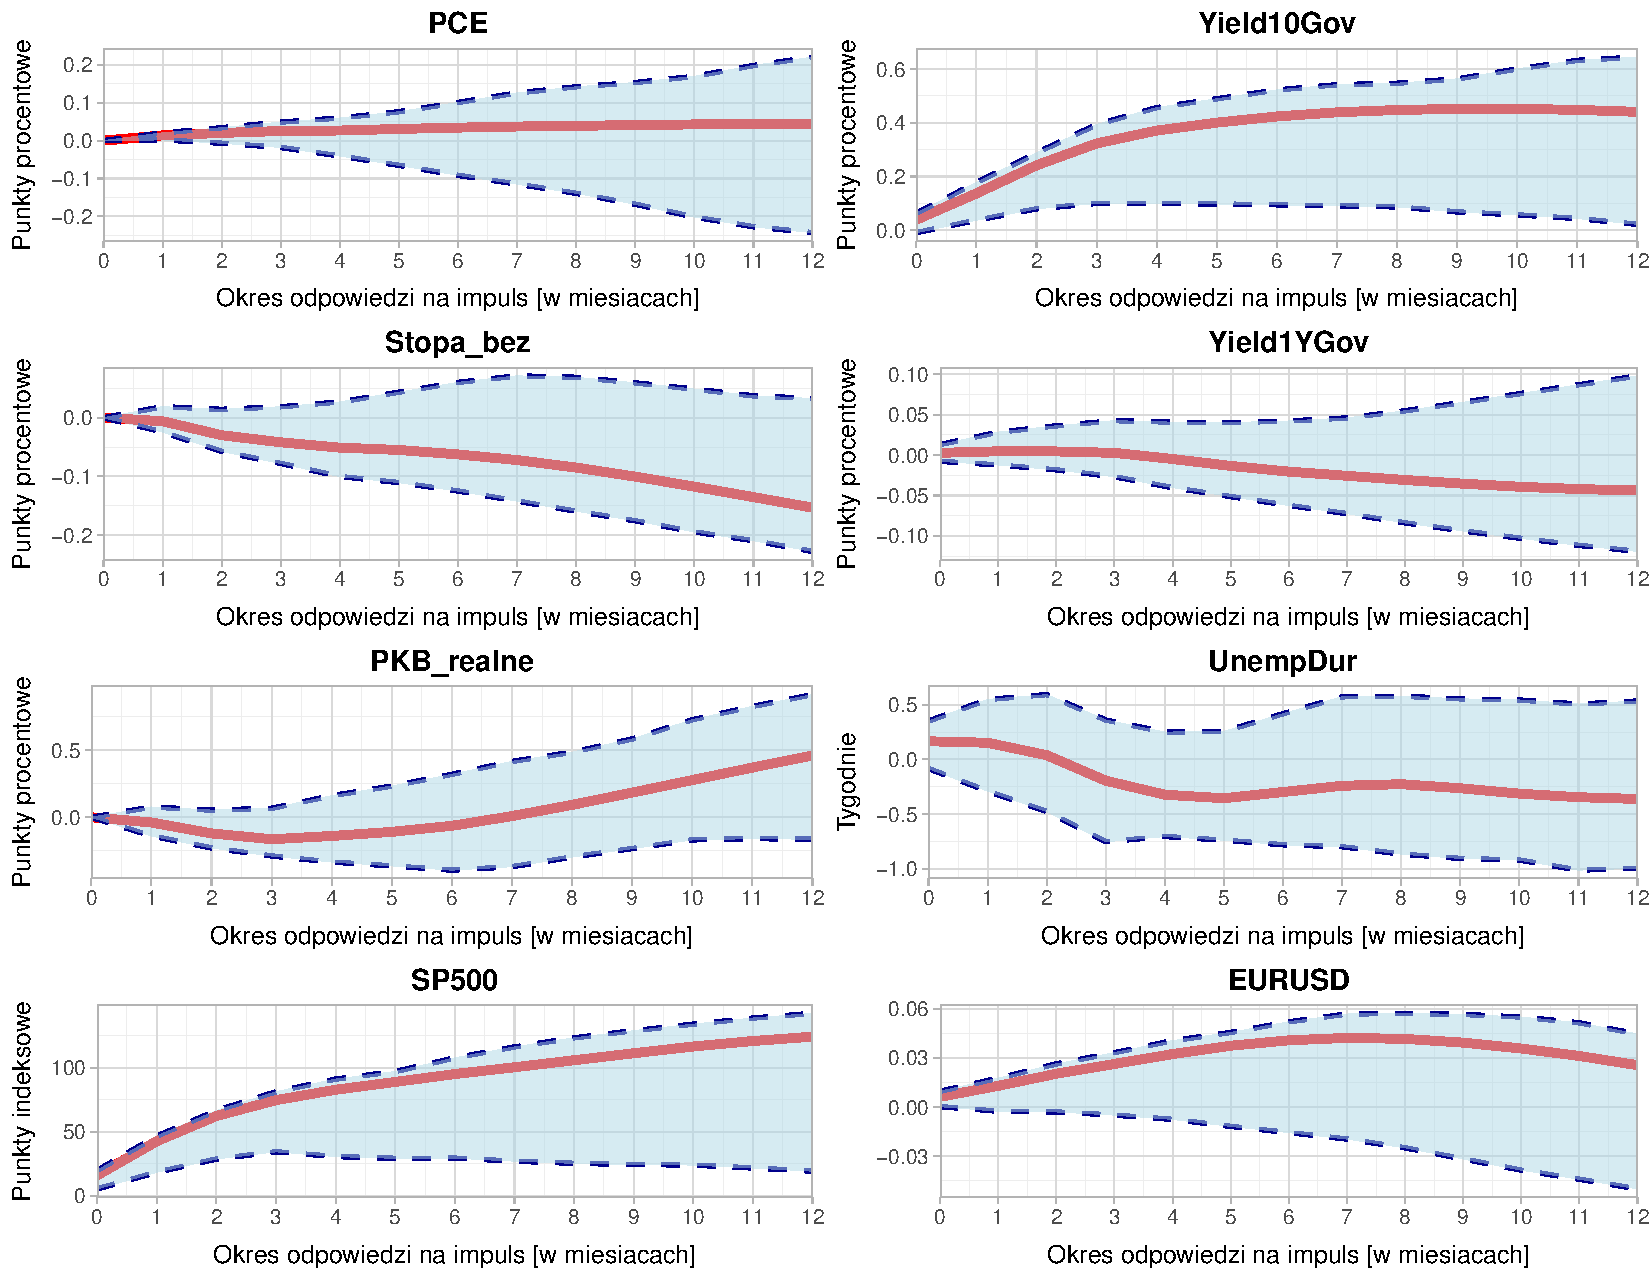
\includegraphics[height=4.8in]{IRFs}
    \captionsetup{format=hang}
    \caption{Funkcje odpowiedzi zmiennych z~modelu VAR na impuls niekonwencjonalnej polityki pieniężnej Rezerwy Federalnej oraz 95\% przedziały ufności tych funkcji.}
\end{centering}
\begin{flushleft}
\vspace{-0.3cm}
\hspace{1cm}\textit{\footnotesize{Źródło: Opracowanie własne.}} \\
\end{flushleft}
\vspace{-0.5cm}
\end{figure}

Wykres reakcji zmiennej \textit{PCE} wskazuje, iż nieoczekiwany wzrost wartości dłużnych instrumentów finansowych skupowanych przez Rezerwę Federalną o~około 120~miliardów dolarów (6\% \acs{PKB} Stanów Zjednoczonych) mógł wpłynąć w~rocznej perspektywie na wzrost wskaźnika cen o~0,05~punktu procentowego (3\% średniej wartości zmiennej w~latach 2008-2016). Kierunek i~skala zmiany zmiennej \textit{PCE} wydaje się wskazywać, iż niekonwencjonalna polityka monetarna Rezerwy Federalnej nie wywarła wielkiego wpływu na poziom cen w~amerykańskiej gospodarce. Nie mniej jednak jest obserwacje te są zgodne z~wnioskami badawczymi odnotowywanymi w~literaturze, gdzie reakcja poziomu cen na niekonwencjonalną politykę monetarną kształtowała się na poziomie od 0,02 p.p. do 0,15 p.p.

Wykres reakcji zmiennej \textit{Yield10Gov} wskazuje, iż innowacja w~polityce monetarnej Rezerwy Federalnej polegająca na zastosowaniu niekonwencjonalnej polityki pieniężnej w~skali około 120~miliardów dolarów mogła doprowadzić do wzrostu dziesięcioletniej krzywej dochodowości o~około 45~punktów bazowych (17\% średniej wartości zmiennej \textit{Yield10Gov}). Takie zachowanie analizowanej zmiennej wydaje się sprzeczne z~oczekiwaniami szefów amerykańskich władz monetarnych - jednym z~ich głównych celów było obniżenie długoterminowych rentowności amerykańskich obligacji skarbowych, tymczasem model \acs{VAR} wskazuje, iż nie tylko nie zrealizowano tego celu, ale efekty ich działań mogły przynieść skutek odwrotny, przynajmniej w~tym fragmencie krzywej dochodowości. Obserwacje te pozostają jednak w~zgodzie z~wnioskami wypływającymi z~pierwszej części rozdziału, gdzie ogłaszanie kolejnych niekonwencjonalnych programów (poza pierwszym z~nich) prowadziło w~krótkoterminowej perspektywie do wzrostu krzywej dochodowości. Jak widać efekt wzrostu rentowności amerykańskich obligacji skarbowych na skutek niekonwencjonalnych działań Rezerwy Federalnej utrzymał się w~okresie dłuższym niż kilka miesięcy i~reakcja ta była silniejsza niż obserwowana w~krótszym terminie. Mogłoby to potwierdzać hipotezę o~odpływie kapitału z rynków dłużnych długoterminowych papierów wartościowych jako reakcji inwestorów na ogłaszanie kolejnych niekonwencjonalnych programów. Obserwacje te jednak, jak już wcześniej wspominano, stoją w~sprzeczności z~literaturą badawczą, gdzie nadzwyczajne działania Rezerwy Federalnej miały prowadzić do statystycznie istotnej obniżki rentowności amerykańskich obligacji skarbowych w skali od 0,05 do 0,5 punktu procentowego. Reakcja krótkiego końca krzywej dochodowości na poziomie około -5~punktów bazowych (14\% średniej rentowności rocznych obligacji) badana przy użyciu zmiennej \textit{Yield1YGov} każe z~kolei przypuszczać, iż nie cała krzywa dochodowości reagowała tak samo na niekonwencjonalną politykę monetarną - bliższy koniec krzywej wydaje się bardziej wrażliwy na działania Rezerwy Federalnej reagując zgodnie z~jej intencjami oraz z~badaniami przestawionymi w~literaturze.

Funkcja odpowiedzi na impuls zmiennej \textit{PKB_realne} pokazuje, że szok w~polityce monetarnej amerykańskich władz monetarnych w~pierwszych sześciu miesiącach mógł wpłynąć na osłabienie wzrostu gospodarczego by w~kolejnych 6~miesiącach doprowadzić do jego umocnienia notując ostatecznie w~rocznej perspektywie pozytywną zmianę na poziomie blisko 50~punktów bazowych (39\% średniej wartości zmiennej w~latach 2008-2016). Taki efekt byłby zbieżny z~oczekiwaniami Rezerwy Federalnej (oraz z~literaturą badawczą), gdyż oznacza realny i~istotny wpływ jej działań na amerykańską gospodarkę, pomimo odwrotnego od zamierzeń wpływu na długoterminową krzywą dochodowości.

Ostatnią istotną funkcją reakcji na szok w~polityce monetarnej jest \acs{IRF} zmiennej \textit{SP500}, gdzie w~perspektywie rocznej umieszczenie przez Rezerwę Federalną 120~miliardów dolarów na rynku dłużnych papierów skarbowych mogło spowodować wzrost indeksu S\&P500 o~około 150 punktów bazowych, czyli ponad 10\% średniej wartości indeksu w~latach 2008-2016. Wiedząc, iż średnia kapitalizacja wszystkich spółek należących do indeksu S\&P500 w~latach 2008-2016 wynosiła około 15~bilionów dolarów, można wyliczyć, iż wzrost indeksu o~10\% oznacza wzrost wycen spółek o~około 1,5~biliona dolarów. Rynek akcji mógłby być więc jednym z~tych rynków, na który odpłynął kapitał z~rynku amerykańskich obligacji skarbowych. Podobne wnioski tylko o~mniejszej oszacowanej skali (0,2-1\% pozytywnego wpływu \acs{MNK} na poziom cen) można odnaleźć w~przedstawionej w~drugim rozdziale literaturze badawczej(\cite{chen36}, \cite{bhattarai36}, \cite{swanson37}).

Reakcje stopy bezrobocia, mediany czasu trwania bezrobocia oraz kursu EUR/USD okazały się nieistotne odnosząc skalę ich reakcji na impuls niekonwencjonalnej polityki monetarnej do ich średnich wartości (odpowiednio -2\%, -2,5\% i~2\%). Wygląda więc na to, iż nadzwyczajne działania Rezerwy Federalnej nie wpłynęły istotnie na rynek pracy oraz rynek walutowy, mogły jednak mieć istotny wpływ na zachowanie się rynków dłużnych papierów skarbowych oraz akcji, a~także poziomu produkcji i~cen w~amerykańskiej gospodarce. Obserwacje te dobrze jest jednak potwierdzić analizą funkcji dekompozycji wariancji błędów prognoz.

\subsection*{\normalsize{Analiza dekompozycji wariancji błędów prognoz finalnego modelu VAR}}

Kolejnym etapem badania relacji pomiędzy zmiennymi w~finalnym modelu wektorowej autoregresji jest analiza dekompozycji wariancji błędów prognoz (ang. \textit{Forecast Error Variance Decomposition - FEVD}). Pozwala ona sprawdzić jaka część wariancji zmiennej jest skutkiem jej własnego szoku, a~jaka wynika z~szoku innych zmiennych, ukazując tym samym dynamikę rozchodzenia się szoków po systemie równań modelu \acs{VAR}. Podobnie jak w~przypadku funkcji \acs{IRF} główny nacisk analizy został położony na wpływ szoku zmiennej \textit{FED_Securities} na pozostałe zmienne wykorzystane w~modelu. \hyperlink{fig15}{Wykres 14} prezentuje dekompozycje wariancji błędów prognoz dla wszystkich zmiennych wykorzystanych w~analizowanym modelu  \acs{VAR}. Jak widać zmienna \textit{FED_Securities} istotnie wpływa na wariancję jedynie dwóch zmiennych (wyłączając jej własną wariancję): \textit{SP500} oraz \textit{Yield10Gov}, w~rocznej perspektywie wyjaśniając odpowiednio: 21\% oraz 14\% ich zmienności. W~przypadku pozostałych zmiennych wpływ ten jest marginalny - nie przekracza 7\%. 

\vspace{0.25cm}
\hypertarget{fig15}{}
\begin{figure}[h]
\begin{centering}
  \hspace{-0.55cm}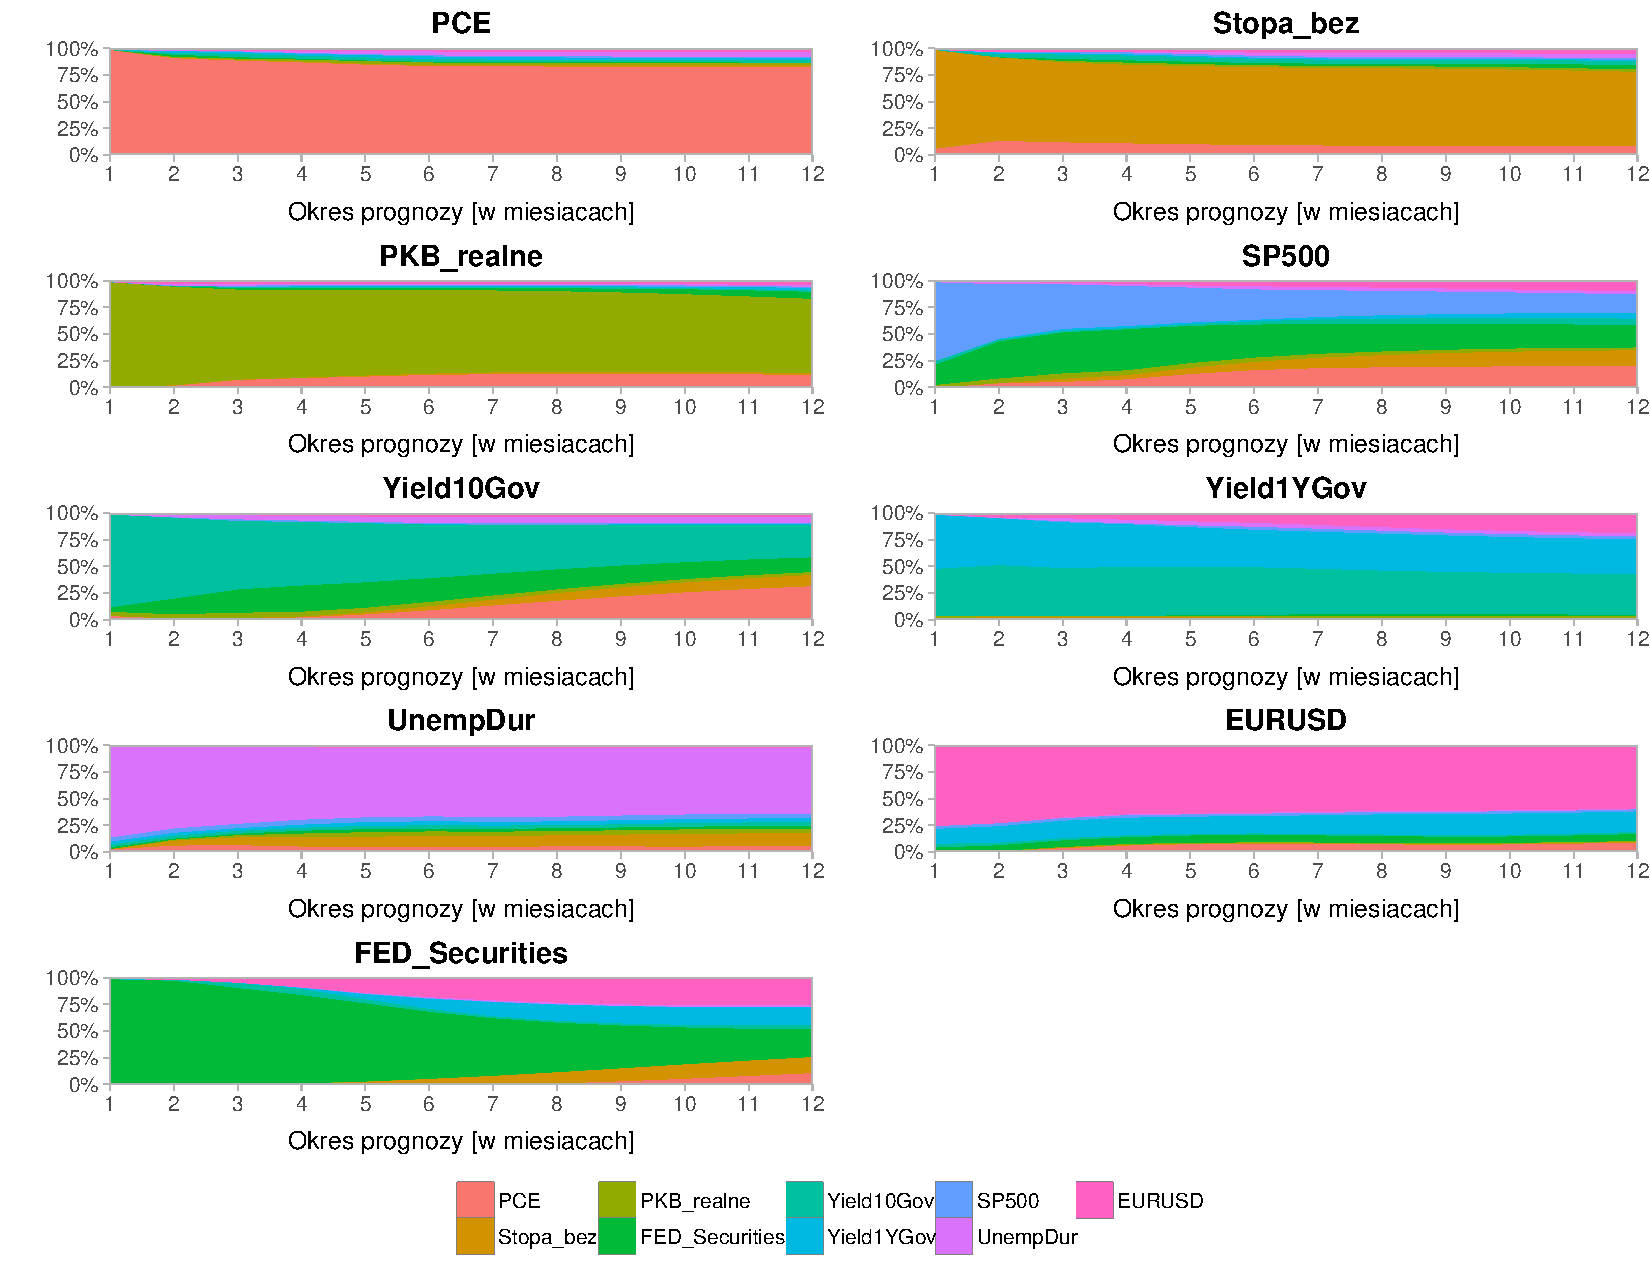
\includegraphics[height=6in, width=6.5in]{FEVDs}
    \captionsetup{format=hang}
    \caption{Dekompozycje wariancji błędów prognoz dla zmiennych z~finalnego modelu VAR}
\end{centering}
\begin{flushleft}
\hspace{1cm}\textit{\footnotesize{Źródło: Opracowanie własne.}} \\
\end{flushleft}
\vspace{-0.5cm}
\end{figure} 

Analizując wykres dekompozycji wariancji indeksu S\&P500 można zaobserwować, iż o~ile w~pierwszym miesiącu na wariancję tej zmiennej wpływa przede wszystkim jej szok własny (74\% zmienności), co jest całkowicie naturalne, to w~perspektywie rocznej najbardziej istotnym czynnikiem kształtującym zmienność tego indeksu jest szok zmiennej reprezentującej wartość papierów dłużnych nabywanych przez Rezerwę Federalną (21\% zmienności przy zaledwie 17\% zmienności wynikającej z~szoku \textit{SP500}). W~przypadku pozostałych analizowanych zmiennych przeważający wpływ w~całym oknie badawczym mają w~przeważającej większości szoki własne tych zmiennych. Takie zachowanie wariancji indeksu S\&P500 może wskazywać na silny wpływ niekonwencjonalnej polityki monetarnej na amerykański rynek akcji w~badanym okresie co wzmacniałoby obserwacje poczynione przy okazji badania funkcji odpowiedzi na impuls. 

Wykres dekompozycji wariancji błędów prognoz dla dziesięcioletnich rentowności amerykańskich obligacji skarbowych wskazuje, iż wpływ szoku niekonwencjonalnej polityki monetarnej na zmienność \textit{Yield10Gov} wynosił od 4\% w~pierwszym miesiącu przez 25\% w~czwartym aż po 14\% w~rocznej perspektywie - konsumując dużą część spadku wpływu zmienności własnej (z~87\% do 31\%). Potwierdza to istotność oddziaływania decyzji amerykańskich władz monetarnych na rynek długoterminowych obligacji skarbowych w~krótkiej i~średniej perspektywie odnotowaną w~poprzednim podrozdziale, a~także przy analizie funkcji odpowiedzi na impuls. Poza wpływem zmiennej \textit{FED_Securities} na \hyperlink{fig15}{wykresie 14} widać również inne istotne powiązania pomiędzy zmiennymi wykorzystanymi w~finalnym modelu wektorowe-autoregresji:
\begin{itemize}
\setlength\itemsep{0.05cm}
\item duży udział szoku na rentowności dziesięcioletnich amerykańskich obligacji skarbowych w~zmienności rentowności obligacji rocznych (od 44\% do 38\%) przy praktycznym braku symetrycznej zależności - co może potwierdzać rolę obligacji dziesięcioletnich jako punktu odniesienia całego rynku obligacji skarbowych,
\item blisko 33\%-owy udział szoku zmiennej \textit{PCE} w~wariancji zmiennej \textit{Yield10Gov} (udział ten jest wyższy nawet od udziału szoku własnego zmiennej 31\%), co może wskazywać na silny wpływ odczytów poziomu cen na kształtowanie się rentowności długoterminowych obligacji,
\item 21\% zmienności S\&P500 zdaje się tłumaczyć szok na wskaźniku cen \textit{PCE} - co wskazywałoby na jego istotność w~procesie decyzyjnym uczestników amerykańskiego rynku akcji,
\item 18\%-owy udział szoku na kursie EUR/USD w~całkowitej wariancji zmiennej \textit{Yield1YGov} przy 20\% relacji odwrotnej, co może być tłumaczone istotnym udziałem podmiotów zagranicznych w~tym fragmencie rynku amerykańskich dłużnych papierów skarbowych,
\item 15\% zmienności S\&P500 zdaje się tłumaczyć szok na wskaźniku bezrobocia \textit{Stopa_bez} - co wskazywałoby na jego istotność w~procesie decyzyjnym uczestników amerykańskiego rynku akcji,
\item 13\% wariancji realnego produktu krajowego brutto tłumaczy zmienność indeksu prywatnych wydatków konsumpcyjnych,
\item około 12\% zmienności średniej długości trwania bezrobocia mogą tłumaczyć szoki na stopie bezrobocia, co wydaje się oczywiste, dziwić może jedynie niska skala wpływu,
\item największy wpływ na wariancję zmiennej \textit{FED_Securities} (poza szokiem jej samej) miały szoki zmiennych: kurs EUR/USD (24\%), rentowność rocznych obligacji skarbowych (17\%), stopa bezrobocia (15\%), roczna zmiana \acs{PKB} realnego (13\%) oraz wskaźnik \acs{PCE} (12\%). Zmienne te pokrywają się z~celami banku centralnego Stanów Zjednoczonych, co nie powinno dziwić w sytuacji, gdy wartość zmiennej \textit{FED_Securities} w~latach 2008-2016 zależała ściśle od decyzji Rezerwy Federalnej. Jednakże kolejność i~istność poszczególnych celów amerykańskich władz monetarnych znacznie się różni się od tej z~dekompozycji wariancji błędów prognoz.
\end{itemize}

Analiza dekompozycji wariancji błędów prognoz potwierdza poprzednie obserwacje dotyczące wpływu niekonwencjonalnej polityki pieniężnej na rynek dłużnych papierów skarbowych oraz rynek akcji. Nie potwierdziły się jednak obserwacje dotyczące wpływu zmiennej \textit{FED_Securities} na poziom produkcji - największy wpływ na wariancje zmiennej \textit{PKB_realne} miały szoki własne tej zmiennej (około 70\% w~rocznej perspektywie). Kolejnym i~zarazem ostatnim etapem badania będzie wygenerowanie prognoz z~finalnego modelu \acs{VAR}, sprawdzenie ich jakości porównując je do wartości rzeczywistych (tzw. \textit{backtesting}) oraz interpretacja rocznych prognoz dla okresu lipiec 2016 - czerwiec 2017.

\subsection*{\normalsize{Analiza prognoz uzyskanych z~finalnego modelu VAR}}

Analizę prognoz uzyskanych z~finalnego modelu wektorowej autoregresji rozpoczęto od przeprowadzenia wstecznych testów jakości prognoz dla lat 2008-2016. W~tym celu dla każdego miesiąca pomiędzy lipcem 2008~a~czerwcem 2016~oszacowano osobny model \acs{VAR}, uzyskując łącznie 96~takich modeli. Starano się przy tym wykorzystywać ośmioletnią próbkę danych dla każdego miesiąca, czego nie udało się osiągnąć dla miesięcy z~lat 2008-2009 ze względu na dostępność danych jedynie od stycznia 2002~roku. Z~tak wyestymowanych 96~modeli wygenerowano następnie roczne prognozy, porównano je z~rzeczywistymi realizacjami zmiennych i~wyliczono dla nich pierwiastki błędów średniokwadratowych. Aby zapewnić porównywalność pomiędzy tymi błędami postanowiono zastosować ich standaryzację - dzieląc je przez ich własną średnią i~otrzymano znormalizowane pierwiastki błędów średniokwadratowych (ang. \textit{Normalized Root-Mean-Square Errors - NRMSE}). Wyliczone miesięczne \acs{NRMSE} dla wszystkich zmiennych zostały zagregowane i~uśrednione do lat (patrz \hyperlink{tab7}{tabela 8}). 

\hypertarget{tab7}{}
\begin{table}[!ht]
\rowcolors{2}{lightgray}{white}
\footnotesize
\captionsetup{format=hang, position=top}
\caption{Błędy NRMSE prognoz finalnego modelu VAR w~latach 2008-2016 (jako \% średniej)}
\begin{tabular}{cccccccccc}
\toprule
\textbf{Year} & \textbf{PCE} & \textbf{\begin{tabular}[c]{@{}c@{}}Stopa\\ bezr.\end{tabular}} & \textbf{\begin{tabular}[c]{@{}c@{}}PKB\\ realne\end{tabular}} & \textbf{\begin{tabular}[c]{@{}c@{}}FED\\ Securities\end{tabular}} & \textbf{\begin{tabular}[c]{@{}c@{}}Yield-\\ 10Gov\end{tabular}} & \textbf{SP500} & \textbf{\begin{tabular}[c]{@{}c@{}}Yield-\\ 1YGov\end{tabular}} & \textbf{\begin{tabular}[c]{@{}c@{}}Unemp-\\ Dur\end{tabular}} & \textbf{EURUSD} \\ \midrule
\textbf{2008} & 56\% & 49\% & 344\%  & 30\%  & 71\%  & 41\%  & 597\%  & 48\% & 89\% \\ 
\textbf{2009} & 68\% & 65\% & 867\% & 60\% & 82\% & 142\% & 225\% & 58\% & 96\% \\
\textbf{2010} & 23\% & 30\% & 326\% & 18\% & 37\% & 16\% & 124\% & 22\% & 18\% \\ 
\textbf{2011} & 23\% & 11\% & 106\% & 24\% & 32\% & 17\% & 129\% & 23\% & 16\% \\ 
\textbf{2012} & 32\% & 12\% & 83\% & 14\% & 20\% & 9\% & 61\% & 21\%  & 11\% \\
\textbf{2013} & 31\% & 6\% & 72\% & 14\% & 33\% & 9\% & 39\% & 21\% & 9\% \\
\textbf{2014} & 23\% & 9\% & 42\% & 15\% & 7\% & 6\% & 35\% & 16\% & 10\% \\ 
\textbf{2015} & 5\% & 4\% & 45\% & 24\% & 17\% & 14\% & 33\% & 12\% & 7\% \\ 
\textbf{2016} & 4\% & 2\% & 47\% & 2\% & 9\% & 6\% & 13\% & 21\% & 4\% \\ 
\textbf{Średnia} & 29\% & 21\% & 214\% & 22\% & 34\% & 29\% & 139\% & 27\% & 29\% \\ 
\bottomrule
\end{tabular}
\begin{flushleft}
\hspace{1cm}\textit{\footnotesize{Źródło: Opracowanie własne.}} \\
\end{flushleft}
\vspace{-0.5cm}
\end{table} 

Analiza \hyperlink{tab7}{tabeli 8}~wskazuje, iż najgorsza jakość prognoz została uzyskana w~2009~roku - był to okres najbardziej gwałtownej zmiany wskaźników gospodarczych, a~najlepsza w~2016~roku, co jest zgodne z~oczekiwaniami, gdyż do tego okresu model był dopasowywany. Jakość prognoz z~roku na rok ulegała poprawie, co pozwala być pozytywnie nastawionym do prognoz na okres z~poza próbki. Większość zmiennych okazała się być prognozowana na dobrym poziomie jakości - średnie błędy \acs{NRMSE} w~96~miesięcznych prognozach nie przekroczyły 30\% dla wszystkich zmiennych poza zmiennymi: \textit{PKB_realne} (214\%) oraz \textit{Yield1YGov} (139\%). Najwyższą jakość prognoz uzyskano z~kolei dla: \textit{FED_Securities} oraz \textit{Stopa_bez}, gdzie w~badaniu dla lat 2008-2016 popełniano błędy na poziomie około 1/5 ich wartości średniej. Jeszcze lepsze wyniki uzyskuje się patrząc na sam 2016~rok, gdzie 2/3 zmiennych jest prognozowana przy błędach nie przekraczający 10\% wartości średniej, a~jedynie \acs{PKB} realne (47\%) wyraźnie negatywnie odstaje od pozostałych wskaźników. W~związku z~tym, iż jakość prognoz modelu wektorowej autoregresji można potraktować jako test dopasowania modelu do danych, takie wyniki dla zmiennej \textit{PKB_realne} skłaniają do osłabienia wniosków wynikających dla tej zmiennej z~analizy funkcji odpowiedzi na impuls i~dekompozycji wariancji błędów prognoz.

\hypertarget{fig16}{}
\begin{figure}[!ht]
\begin{centering}
  \hspace{-0.55cm}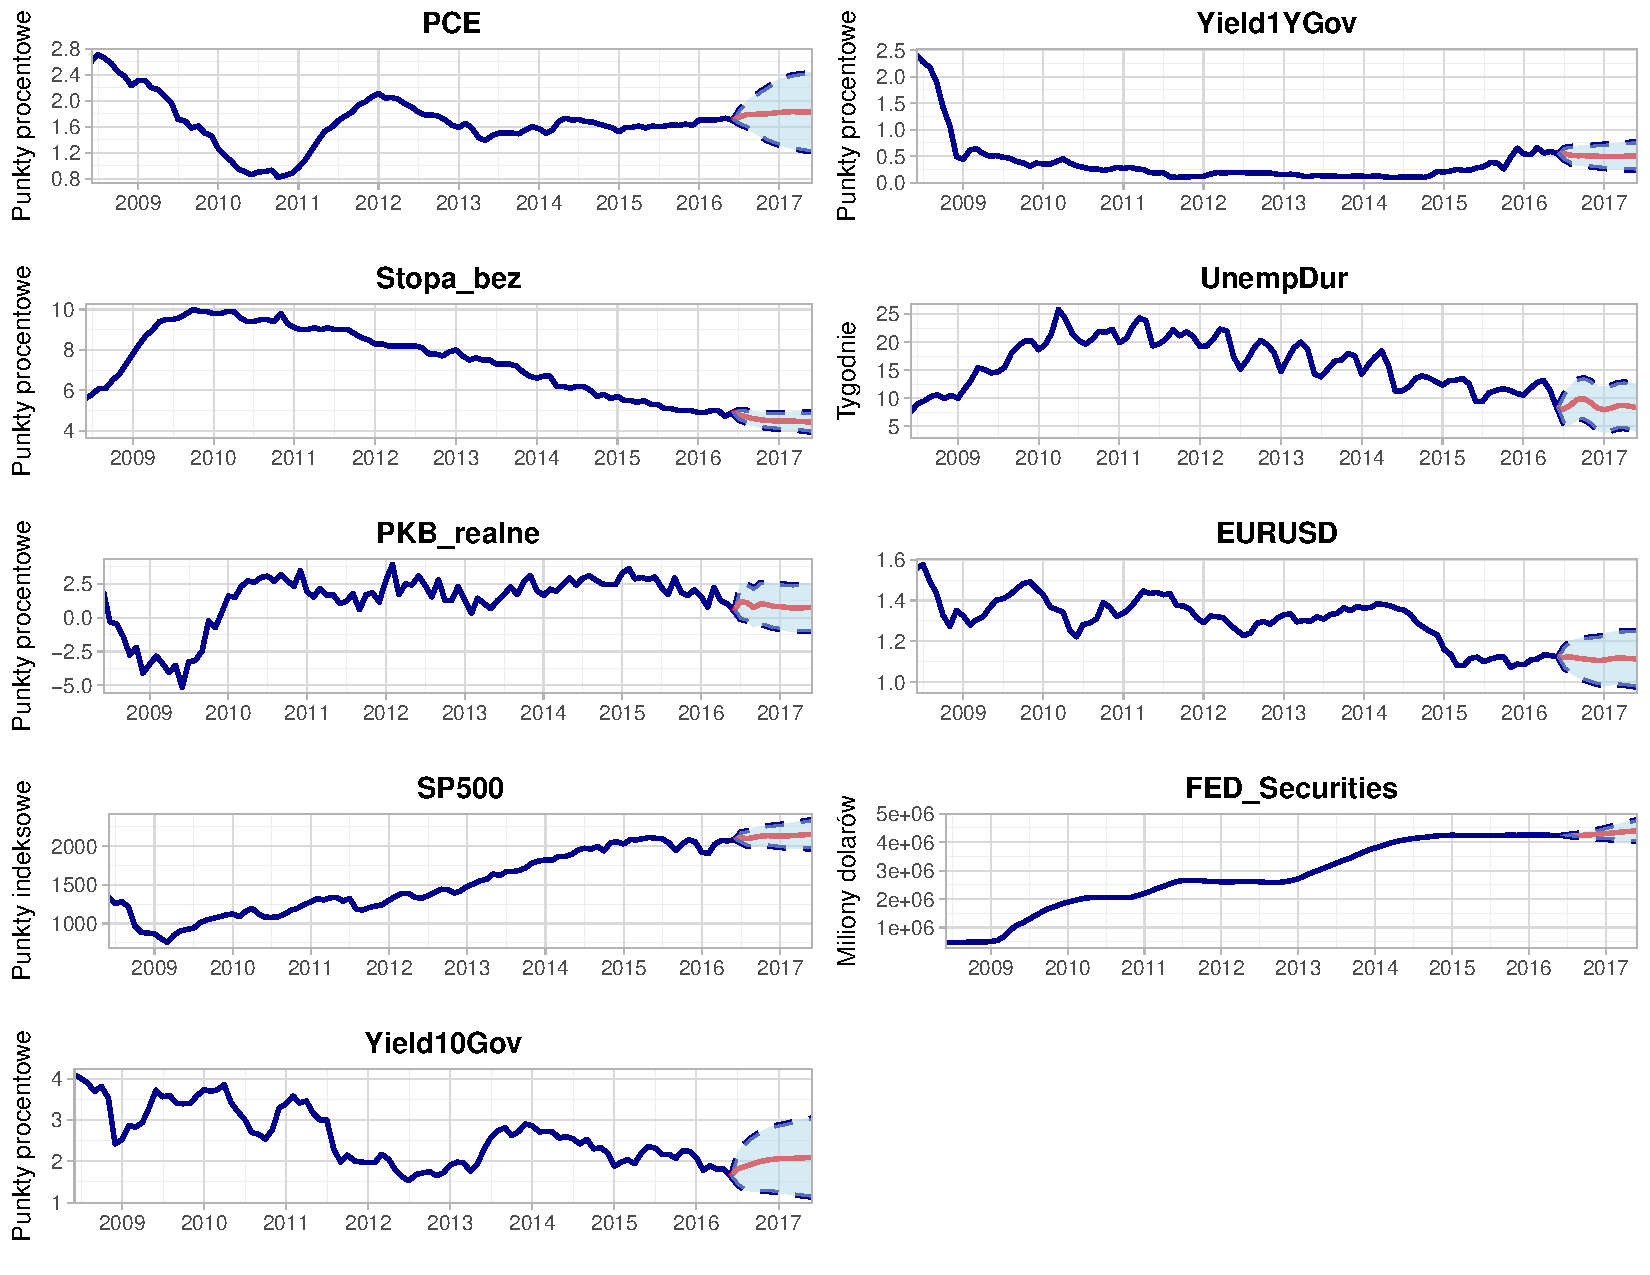
\includegraphics[height=6in, width=6.5in]{Progs}
    \captionsetup{format=hang}
    \caption{Roczne prognozy zmiennych z~finalnego modelu wektorowej autoregresji dla okresu lipiec 2016 - czerwiec 2017 oraz 95\% przedziały ufności tych prognoz}
\end{centering}
\vspace{-0.5cm}
\begin{flushleft}
\hspace{1cm}\textit{\footnotesize{Źródło: Opracowanie własne.}} \\
\end{flushleft}
\vspace{-0.5cm}
\end{figure}

\hyperlink{fig16}{Wykres 15} prezentuje roczne prognozy finalnego modelu wektorowej autoregresji wygenerowane dla wszystkich zmiennych oraz 95\% przedziały ufności tych prognoz wyznaczone za pomocą metody \textit{bootstrap}. Okres prognozy obejmuje 12~miesięcy od lipca 2016~roku do czerwca 2017. Najważniejsze wnioski płynące z~analizy wykresów tych prognoz to:

\vspace{-0.15cm}
\begin{itemize}
\setlength\itemsep{0.05cm}
\item wzrost w~ciągu roku wskaźnika \acs{CPI} z~poziomu 1,6\% do 1,8\% - kontynuacja wzrostu cen w amerykańskiej gospodarce,
\item pogłębienie spadku stopy bezrobocia z~4,9\% w~czerwcu 2016 do 4,6\% w~czerwcu~2017,
\item stabilizacja rocznej zmiany \acs{PKB} realnego na poziomie nie przekraczającym jednego punktu procentowego,
\item powolny wzrost wartości papierów dłużnych w~bilansie Rezerwy Federalnej (200 miliardów dolarów w~ciągu roku),
\item wzrost rentowności dziesięcioletnich amerykańskich obligacji skarbowych od 1,6\% do 2\% oraz stabilizacja rocznych rentowności na poziomie 0,5\%,
\item wzrost wartości indeksu S\&P500 o~ponad 100 punktów indeksowych,
\item stabilizacja mediany czasu trwania bezrobocia w~okolicach~8 tygodni,
\item delikatne umocnienie się dolara w~stosunku do euro - spadek kursu EUR/USD z~poziomu 1,12 do około 1,1. 
\end{itemize}

\noindent Analiza prognoz wygenerowanych z~finalnego modelu wektorowej autoregresji wskazuje w~przypadku większości zmiennych na stabilizację ich wartości w~rocznej perspektywie lub kontynuację dotychczasowych trendów. Najbardziej wartościowymi obserwacjami wydają się prognoza dalszego wzrostu poziomu cen oraz spadku stopy bezrobocia przy stabilizacji rocznej zmiany \acs{PKB} realnego na relatywnie niskim poziomie. Warto pamiętać jednak, iż zmienne \textit{PKB_realne} oraz \textit{Yield1YGov} generowały najwyższe wartości błędów \acs{NRMSE} we wstecznych testach jakości prognoz (kilkukrotnie przekraczające dopuszczalny poziom 30\%), dlatego więc ich prognozy mogą być obarczone dużą skalą niedokładności, związaną z~niewystarczającym dopasowaniem modelu \acs{VAR} dla tych zmiennych. 

\subsection*{\normalsize{Weryfikacja hipotez badawczych}}

W~niniejszym rozdziale zaprezentowano badanie dotyczące wpływu niekonwencjonalnej polityki pieniężnej amerykańskich władz monetarnych na rynek dłużnych papierów skarbowych w~Stanach Zjednoczonych oraz na wskaźniki gospodarcze reprezentujące najistotniejsze segmenty amerykańskiej gospodarki. Główną hipotezą badawczą pracy było stwierdzenie, iż niekonwencjonalna polityka monetarna Rezerwy Federalnej stosowana od 2008~roku zamiast pobudzać do wzrostu realnego \acs{PKB} oraz~zbliżać amerykańską gospodarkę do pełnego zatrudnienia przyczyniła się przede wszystkim do wygenerowania ponadprzeciętnych wzrostów cen akcji notowanych na giełdach w~Stanach Zjednoczonych. Tak sformułowana hipoteza badawcza zakładała nie tylko brak pełnej efektywności kanałów transmisji monetarnej w~przekazywaniu impulsów polityki pieniężnej do realnej gospodarki, ale również strukturalną ułomność kanału kredytowego oraz kanału cen akcji, które pomimo ogromnej stymulacji monetarnej realizowanej poprzez działania banku centralnego, zamierzonej w~przypadku kanału kredytowego oraz niezamierzonej (a~przynajmniej nie deklarowanej) w~przypadku kanału cen akcji, nie przekazały adekwatnie silnego impulsu wzrostowego do amerykańskiej gospodarki. Celem badania zrealizowanego w~tej części pracy było zweryfikowanie przedstawionej hipotezy.

Wyniki badania zaprezentowanego w~pierwszej części omawianego rozdziału wskazują, iż amerykański bank centralny implementując niekonwencjonalne programy polityki monetarnej wpływał istotnie na rynek dłużnych papierów skarbowych w~Stanach Zjednoczonych jednak wpływ ten był zgodny z~intencją banku tylko w~przypadku pierwszego luzowania ilościowego (istotne statystycznie obniżenie rentowności amerykańskich obligacji skarbowych na całej długości krzywej dochodowości). W~przypadku ogłaszania kolejnych niekonwencjonalnych programów oraz w~trakcie ich trwania rentowności amerykańskich obligacji skarbowych reagowały wzrostami lub nie zmieniały istotnie swoich wartości. Wszelkie informacje dotyczące zakończenia tych programów prowadziły natomiast do wzrostów tych rentowności. Aby potwierdzić te obserwacje w~kolejnej części niniejszego rozdziału wyestymowano model wektorowej autoregresji zawierający wskaźniki gospodarcze reprezentujące najistotniejsze segmenty gospodarki Stanów Zjednoczonych.

Wyniki modelu \acs{VAR} przedstawione \hyperlink{podrz32}{w~podrozdziale 3.2.} wskazują na statystycznie istotny, nieobciążony błędami i~silnie oddziałujący wpływ niekonwencjonalnej polityki pieniężnej na tylko dwa segmenty amerykańskiej gospodarki: rynek akcji (reprezentowany przez indeks S\&P500) oraz rynek długoterminowych dłużnych papierów skarbowych (reprezentowany przez rentowność dziesięcioletnich obligacji skarbowych). Analiza tego wpływu na pozostałe segmenty amerykańskiej gospodarki wskazała, iż albo jest on marginalny w~odniesieniu do średniej wartości zmiennej reprezentującej dany segment, albo nie wpływa on istotnie na zmienność danego wskaźnika sektorowego, lub też generuje wysokie wartości błędów prognoz. Może to oznaczać brak istotnego wpływu niekonwencjonalnych działań Rezerwy Federalnej na gospodarkę Stanów Zjednoczonych co wskazywałoby na brak pełnej efektywności kanałów transmisji niekonwencjonalnej polityki monetarnej w~Stanach Zjednoczonych w~latach 2008-2016. 

Analizując wpływ niekonwencjonalnych działań amerykańskich władz monetarnych w~latach 2008-2016 na rynki akcji w~Stanach Zjednoczonych posłużono się funkcją odpowiedzi na impuls polityki monetarnej indeksu S\&P500, która wskazała, iż wzrost wartości zakupionych przez Rezerwę Federalną obligacji o~120~miliardów dolarów mógł spowodować wzrost wartości analizowanego indeksu o~około 150 punktów (10\% jego średniej wartości indeksu w~latach 2008-2016) w~perspektywie rocznej. Z~kolei dekompozycja wariancji błędów prognoz pokazała, iż najistotniejszym czynnikiem (istotniejszym nawet od przeszłych wartości indeksu) kształtującym 20\% zmienności S\&P500 od 2008~roku była niekonwencjonalna polityka Rezerwy Federalnej. Patrząc na wyniki tych analiz oraz wiedząc, iż~10\% wartości analizowanego indeksu odpowiadało w~latach 2008-2016 średnio około 1,5 biliona dolarów można przypuszczać, iż to właśnie rynek akcji wchłonął większość kapitału odpływającego z~rynku dłużnych papierów wartościowych co potwierdziłoby hipotezę główną niniejszej pracy.

Badając wpływ niekonwencjonalnych działań Rezerwy Federalnej w~latach 2008-2016 na rynek długoterminowych dłużnych papierów skarbowych posłużono się funkcją \acs{IRF}, która wskazała, iż wzrost skali niekonwencjonalnej polityki pieniężnej Rezerwy Federalnej o~120~miliardów dolarów mógł doprowadzić do wzrostu rentowności dziesięcioletnich obligacji skarbowych o~około 45~punktów bazowych w~rocznej perspektywie, co ostatecznie potwierdziło wnioski płynące z analizy przeprowadzonej \hyperlink{podrz31}{w~podrozdziale 3.1.} odnośnie odwrotnej od intencji Rezerwy Federalnej reakcji krzywej dochodowości na działania amerykańskiego banku centralnego oraz o~odpływie kapitału z~rynku dłużnych papierów skarbowych. Funkcja dekompozycji wariancji błędów prognoz wskazała z~kolei, iż w~rocznej perspektywie 14\% zmienności rentowności dziesięcioletnich obligacji skarbowych może być wyjaśnione zmiennością skali zakupów dłużnych papierów skarbowych przez Rezerwę Federalną (przy 31\%-owym poziomie wyjaśniania zmiennością własną). Nie jest to oczywiście tak istotny wynik jak w~przypadku indeksu S\&P500 ale pokazuje równie silny wpływ amerykańskich władz monetarnych na ten segment gospodarki Stanów Zjednoczonych.

Porównując uzyskane wyniki z~wynikami przedstawionymi w~artykułach badawczych omówionych w~drugim rozdziale można stwierdzić, iż zgadzają się one ze sobą jedynie częściowo. W~obu z~nich podkreślony zostaje wpływ niekonwencjonalnej polityki monetarnej na rynek akcji w~Stanach Zjednoczonych, jednak oszacowany w~niniejszej pracy wpływ okazał się silniejszy niż ten przedstawiony w~literaturze badawczej. Z~kolei wpływ niekonwencjonalnych działań Rezerwy Federalnej na kształt krzywej dochodowości oszacowany w~niniejszej pracy zdecydowanie różni się od tego przedstawionego w~artykułach badawczych. Autorzy części omówionych w~drugim rozdziale badań przekonują, iż rentowności długoterminowych amerykańskich obligacji skarbowych spadły na skutek niekonwencjonalnej polityki monetarnej prowadzonej przez amerykańskie władze monetarne, w~bieżącej pracy oszacowano, iż zachowanie tych rentowności było całkowicie odwrotne (istotny wzrost rentowności obligacji skarbowych na skutek \acs{NPM}) - wyłączając okres pierwszego luzowania ilościowego.

Wyniki zaprezentowanego w~niniejszym rozdziale badania wskazują na konieczność potwierdzenia głównej hipotezy badawczej niniejszej pracy w~zakresie zaledwie połowicznym - niekonwencjonalna polityka monetarna wpłynęła statystycznie istotnie na wygenerowanie ponadprzeciętnych wzrostów na amerykańskich rynkach akcji. Wpływ nadzwyczajnych działań Rezerwy Federalnej na gospodarkę Stanów Zjednoczonych nie jest tak jednoznaczny. Z~jednej strony oszacowany model \acs{VAR} nie ukazał istotnego wpływu \acs{NPM} na takie zmienne jak stopa bezrobocia, \acs{PCE}, kurs walutowy czy długość trwania bezrobocia, z~drugiej strony istotny wynik dotyczący \acs{PKB} realnego może okazać się obarczony błędami ze względu na słabe dopasowanie modelu. Wygląda więc na to, iż zweryfikowanie tej części hipotezy badawczej wymaga przeprowadzenia dodatkowych badań.